\documentclass[10pt]{report}
\usepackage{lingmacros}
\usepackage[normalem]{ulem}
%  Title Formatting 
\usepackage{titlesec}
% Removes paragraph indenting
\usepackage{parskip} 

% Figure labeling
\usepackage{hyperref}

\usepackage{amsmath}

% Font
\usepackage{tgpagella}

% Inline code
\usepackage{listings, lstautogobble, newtxtt}
\lstset{basicstyle=\ttfamily, keywordstyle=\bfseries}

\usepackage[labelfont=bf, labelsep=period]{caption}
\usepackage{graphicx}
\graphicspath{ {./images/} }

% Makes citations superscript
\usepackage[superscript,biblabel]{cite}
\usepackage{url}
\urlstyle{same}

\titleformat{\chapter}[block]
{\normalfont\huge\bfseries}{\thechapter.}{1em}{\Huge}
\titlespacing*{\chapter}{0pt}{-19pt}{0pt}

\lstset{language=Java,
	showstringspaces=false,
	breaklines=true,
	frameround=ffff,
	frame=single,
	autogobble=true
}


\begin{document}
	\begin{titlepage}
		\begin{center}
			\Large
			\textbf{Procedural Content Generation Using Noise}
			
			\vspace{1.5cm}
			\normalsize
			\textbf{Michael Li}
			
			\vfill
			
			\textbf{DRAFT 4.5.1}
			
			\uline{Dianne Hansford, Ph.D \hfill Director}
			\vspace{1cm}
			
			\uline{Yoshihiro Kobayashi, Ph.D \hfill Second Committee Member}
			
			\vspace{3cm}
			
			
\includegraphics[scale=.5]{asu_barretthonors_horiz_rgb_maroongold_600ppi}
			
			\vspace{1.5cm}
			Ira A. Fulton Schools of Engineering
			
			School of Computing, Informatics, and Decision Systems Engineering
			
			Spring 2021
			
		\end{center}
	\end{titlepage}
	
	\chapter*{Abstract}
	
	\addcontentsline{toc}{chapter}{Abstract}
	Procedural content generation refers to the creation data algorithmically using controlled randomness. These algorithms can be used to generate complex environments as opposed to manually creating environments, using photogrammetry, or other means. Procedurally generated content can be created using noise based algorithms. This paper will detail procedural generation of content using noise.
	
	\clearpage
	
	\tableofcontents
	
	\clearpage
	
	\let\clearpage\relax
	\chapter{Introduction}
		
		Procedural generation is an often hidden, yet common feature among digital content, as it automates the creation of large amounts of data. Often, this is hidden in the backgrounds of movies and video games, as well as other art -- adding subtle texture and variation. Procedural generation has many possible outputs, with some examples being the generation of stories, histories, particle effects, and characters. One of the most famous cases of procedural generation for entire worlds is Minecraft \cite{minecraft-gen}. Other examples of procedural generation's varied uses include games such as The Elder Scrolls II: Daggerfall, which employs various forms of procedural generation to determine the location of non-player characters, the layout of dungeons, as well as the terrain itself \cite{daggerfall}. In more complex cases, procedural generation is used to create fake histories, with the more well-known example of Dwarf Fortress \cite{df-dev}. However, procedural generation's applications are not only limited to games. In The Lord of the Rings, many of the scenes with large amounts of characters were created using procedural generation, ensuring individual animations of the slightly differentiated characters \cite{massive}.
		
		This paper explains procedural algorithms involving noise, and noise's application in generating geological formations and the surrounding terrain. Procedurally generated content (PGC) refers to the use of computers to algorithmically create data using a pseudo-random procedural algorithm, which is then interpreted into content. Some examples of procedural algorithms to create content include noise, fractals, as well as cellular automata. These algorithms can be mixed and matched in any number of ways to fine-tune different outcomes, or to add variety to content. To qualify as PGC, the algorithm to create data must be modifiable and controllable, while the results from the algorithm must be reproducible. The reproducible criteria for PGC can be fulfilled by the use of deterministic random number generators (See \autoref{subsec:rng}), but some forms of procedural algorithms are majority governed by randomness. The modifiable criteria is fulfilled by the use of parameters to modify the algorithm. A deterministic system is a system in which no randomness is involved, while a stochastic system is one that can be described by a random probability distribution. While these concepts may seem to be mutually exclusive, they occupy different portions of the overall procedural generation pipeline, allowing them to co-exist. A geological formation, is a body of rock that possesses some degree of internal consistency or distinctive features \cite{2005}. This allows geological formations to be separate from the region it is placed in while still being a landmark for the region as a whole. Just as sand is individually different at a small scale, so too is the data created by procedural generation. However, when viewed as a whole, there is little difference between each grain. This necessitates user control and adjustments in order to make a region stand out versus another, with the use of landmarks or geological formations.
		
		While noise is the focus of this paper, it is important to note that there are alternatives to noise for creating PGC. One example of this is fractal-based algorithms. Fractals are characterized by their self-similarity. This means that the parts of the whole fractal contain the same characteristics.
		
		\begin{enumerate}
			\item Draw an Equilateral triangle
			\item Replace all lines as follows, and repeat 2
		\end{enumerate}
		
		\begin{minipage}{\textwidth}
			\centering
			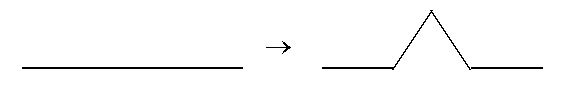
\includegraphics[scale=0.5]{m_reprule}
			\captionof{figure}{Rule of the Koch snowflake \cite{fractal-landscapes}.}
			\label{fig:m_reprule}
		\end{minipage}
		
		After several iterations of this rule, \autoref{fig:m_koch} is the result.
		
		\begin{minipage}{\textwidth}
			\centering
			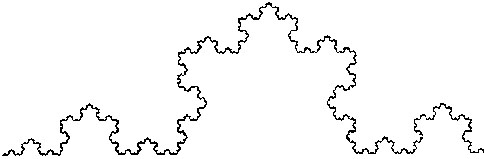
\includegraphics[scale=0.5]{m_koch}
			\captionof{figure}{Koch snowflake \cite{fractal-landscapes}.}
			\label{fig:m_koch}
		\end{minipage}
	
		The rule described for the creation of the Koch snowflake can be repeated endlessly. Fractals and the subsequent geometric shapes that can be created from fractals were found to be useful in describing nature. By studying geographical data, many similarities such as self-similarity and the subdivision of space were found, pushing the study of fractal geometry forward \cite{doi:10.1111/j.1467-8306.1987.tb00158.x}. 
		
		Another method of generating terrain and other features such as caves \cite{10.1145/1814256.1814266} revolves around the use of cellular automata. Cellular automata are a model of a system of cell objects with three characteristics. The cells must be placed on a regularly spaced grid, regardless of dimensionality. These cells must each have a state, which can describe any number of features for each individual cell. Lastly, each cell must have a neighborhood. While typically a neighborhood is composed of only the adjacent cells, it can be defined in any number of ways. This approach relies on having the information of neighbors and the states of their neighbors to determine surrounding cells to then modify their states \cite{nature-of-code}. 
		
		\begin{minipage}{\textwidth}
			\centering
			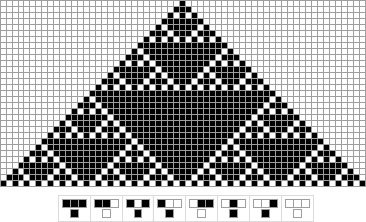
\includegraphics[scale=0.7]{rule-30}
			\captionof{figure}{1-Dimensional cellular automata example. Each row is an iteration, following the eight rules at the bottom \cite{cell-30}.}
			\label{fig:cell-30}
		\end{minipage}
		
		\begin{minipage}{\textwidth}
			\centering
			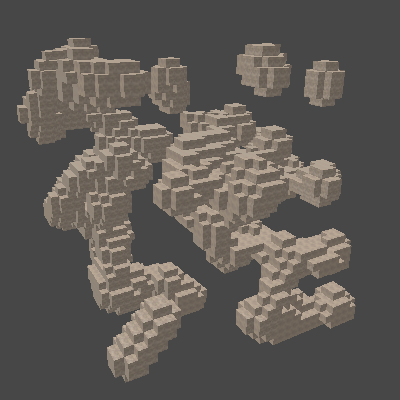
\includegraphics[scale=.6]{cellular-automata-cave}
			\captionof{figure}{An example of three-dimensional cellular automata cave generation \cite{bergauer_prozedurale_nodate}}
			\label{fig:ca-cave}
		\end{minipage}
		
		\section{Motivation for Procedurally Generated Content}
		
		Topography is the study of the land surface, encompassing both natural and artificial features covering the surface. Procedural generation is often used in the creation of features such as geological formations and topography due to the self-similarity found in nature. While fractals serve as a good description of the fractal properties of edge-like features, such as the length of coastlines \cite{ijgi5060095}, noise can also generate these features, as well as filling out the areas in between more easily than fractal algorithms. While creating these features is possible through other means, such as by hand or through photogrammetric methods \cite{bullinger2020photogrammetrybased}, using procedural algorithms allows for easier control over much larger surfaces, and can lead to similar quality results with the reduction of manual labor. This allows for smaller teams to more easily populate and create densely featured worlds. Some examples of this can be found in the procedural coverage and generation of vegetation of terrain, respectively, using custom built tools \cite{redengine}, or tools such as World Machine \cite{world-machine}. Another common example of procedural generation is hidden in the backgrounds of movies, with procedural algorithms populating the topography in Pixar movies \cite{10.1145/3388767.3407372}.
		
		\section{Fundamentals} 
			\subsection{Random Numbers} \label{subsec:rng}
		
			PGC is often dependent on the use of random numbers.The generation of random numbers is difficult as the algorithm or process used to obtain random numbers must not output random numbers with any recognizable patterns or regularities. This property is know as statistical randomness. Statistical randomness ensures that the probability distribution is uniform, with any number in the given range having an equal change of being selected. Random numbers may be generated non-deterministically through the interpretation of unpredictable physical processes, and deterministically using an algorithm \cite{rng}. These methods are also known as random bit generators, Non-deterministic Random Bit Generators (NRBG) and Deterministic Random Bit Generators (DRBG), respectively. One example of an unpredictable physical process to generate non-deterministic random numbers is through using radio receivers to pick up atmospheric noise \cite{random-org}. A NRBG measures a random physical process such as atmospheric noise and compensates for potential biases to generate a random number. While it is "theoretically impossible to prove that a random number generator is really random," the numbers produced by the generator can be analyzed to increase or decrease confidence in the generator \cite{random-org}. For deterministically generated random numbers the random numbers are algorithmically determined using an input value (also known as a seed). A DRBG is an algorithm to generate a sequence of numbers whose distribution approximates a sequence of random numbers. The algorithm to create these numbers is static -- by inputting a seed, the same sequence of random numbers will always be created. This property of seeding differentiates a DRBG and a NRBG. While a DRBG's outputs are not truly random, the output values in the long term should approximate a NRBG's results. 
			
			The concept of reproducibility is shared between PGC and DRBG's. DRBG's are also known as pseudorandom number generators; the generated numbers from DRBG's are described as pseudorandom because they only approximate randomness \cite{rng}. This is due to the necessity of the seeding value, ensuring the deterministic portion of the definition. PGC algorithms follow the same methodology as DRBGs. PGC also often uses a seed for the procedural algorithm. While not all procedural generation uses a seeding function, seeding is a common property among PGC. In procedural algorithms, an input seed ensures the reproducibility. This seed number will only have meaning in the context of the same algorithm it is being used in -- changing the algorithms and/or manipulating the seed will change the entire output, so reproducibility is often limited to a per-version context. This ensures regularity as well as controlled randomness to the PGC. Procedural algorithms often use more than one random number, as in the case of Perlin noise. By using a seed number to determine the initial state of the DRBG, the sequence of random numbers is fixed for use by the procedural algorithm. 
			
			\begin{lstlisting}[label={lst:np.random}, language=Python, frame=none, caption={An example of seeding NumPy's random function in Python}, captionpos=b]
				import numpy as np
				
				np.random.seed(10)
				np.random.rand(10)
			\end{lstlisting}
			
			For example, in \autoref{lst:np.random}, the same ten digits [0.77132064, 0.02075195, 0.63364823, 0.74880388, 0.49850701, 0.22479665, 0.19806286, 0.76053071, 0.16911084, 0.08833981] will always be returned, in order, because of the use of 10 as the seed for the DRBG. By using a DRBG, the creation of these numbers will be static, as the "seed" for a DRBG will determine the sequence of random numbers that it returns.
			
	\vspace{10pt}
	\let\clearpage\relax
	\chapter{Noise}
		
		A procedural algorithm using noise returns a value in the range of \([0,1]\) for a given coordinate location. By setting a seed, the algorithm's results are reproducible. For this paper, the process of Perlin noise and its derivatives will be focused on, but other methods of generating noise include value noise and Worley noise. Perlin noise and Simplex noise are examples of gradient noises, which are based around lattices. A lattice is a regularly spaced array of points in a square/cube array \cite{integer-lattice}. In one dimension, this appears as a number line. 
		
		\begin{minipage}{\textwidth}
			\centering
			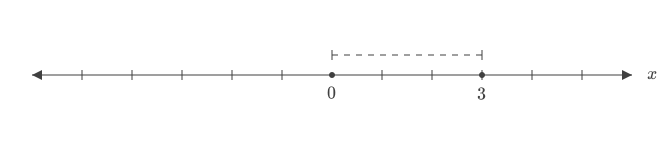
\includegraphics[scale=.4]{1d}
			\captionof{figure}{One-dimensional Integer Lattice \cite{cartesian}}
			\label{fig:1d}
		\end{minipage}
	
		In two dimensions, this becomes a Cartesian coordinate plane in two dimensions.
	
		\begin{minipage}{\textwidth}
			\centering
			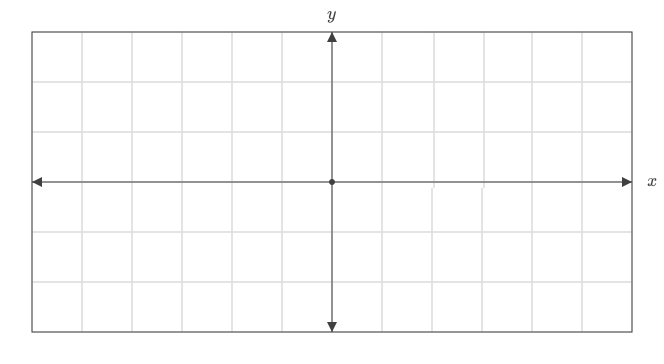
\includegraphics[scale=.35]{2d}
			\captionof{figure}{Two-dimensional Integer Lattice \cite{cartesian}}
			\label{fig:2d}
		\end{minipage}
	
		In three dimensions, this becomes a Cartesian coordinate system in three dimensions.
		
		\begin{minipage}{\textwidth}
			\centering
			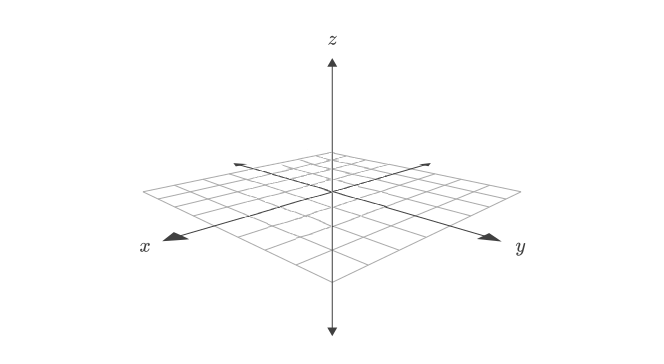
\includegraphics[scale=.5]{3d}
			\captionof{figure}{Three-dimensional Integer Lattice \cite{cartesian}}
			\label{fig:3d}
		\end{minipage}
	
		The dimensionality of Perlin noise and Simplex noise can extend to n-dimensions. These lattices form the basis of Perlin noise.
		
		Interpolation is another concept integral to Perlin noise. Interpolation estimates the value between two points. For example, using linear interpolation and given the two points (1,1) and (3,3), the assumption would be a linear slope between these two points. 
		
		\begin{minipage}{\textwidth}
			\centering
			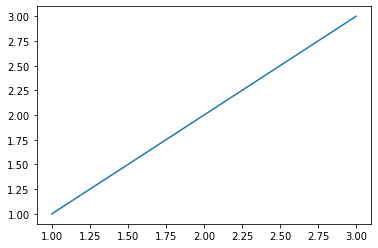
\includegraphics[scale=.5]{linear-interpolation}
			\captionof{figure}{Plot of the two points (1,1) and (3,3), as well as a linear function between the two}
			\label{fig:linear-interpolation}
		\end{minipage}
	
		If asked to estimate the y-value of \(x = 2\), the result would be \(2\), due to the linear interpolation formula.
		
		\[y = \frac{y_0 (x_1 - x) + y_1 (x - x_0)}{(x_1 - x_0)}\]
		
		This linear interpolation function can also be implemented in code, known as the \lstinline|lerp| function, short for linear interpolation. 
		
		\begin{lstlisting}[label={lst:lerp}, language=Python, frame=none, caption={lerp function in Python.}, captionpos=b]
			def lerp(low, high, t):
				return low * (1-t) + high * t
		\end{lstlisting}
		
		Linear interpolation is not the only form of interpolation. Two other forms of interpolation commonly used for Perlin noise include cosine interpolation as well as smoothstep interpolation. The implementation of the smoothstep function will be expanded on in \ref{sec:1d}.
		
		\begin{minipage}{\textwidth}
			\centering
			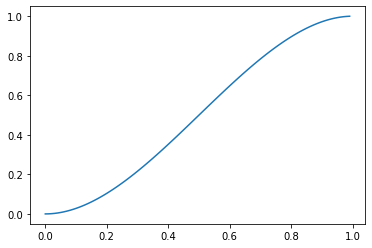
\includegraphics[scale=.5]{smoothstep}
			\captionof{figure}{Example of smoothstep interpolation between two points}
			\label{fig:smooth}
		\end{minipage}
		
		\section{1-Dimensional} \label{sec:1d}
		
		For one-dimensional Perlin noise, the associated lattice will be a number line. At each of the integer \(x\) coordinates, a pseudo-random value is generated. This value represents a gradient, or a slope, at each of the integer coordinates. This gives Perlin noise the category of gradient noise, as opposed to if the values were simply interpreted as values, as in value noise. For simplicity, this pseudo-random gradient value will be represented by \(y\). In one dimension, gradients are one dimensional as well. Since computers do not have infinite storage, either a limit will be imposed to the number of coordinate-value pairs being generated at a time, or the noise algorithm will loop, and set the last coordinate's next coordinate to be the first coordinate, or a hashing function can be used (\ref{subsec:hashing}). The goal is to determine the \(y\) value at a coordinate, or set of coordinates at a non-integer \(x\) coordinate.
		
		Since arbitrary input \(x\) coordinate can have difference distances from the two closest integer coordinates, the influence of the gradient value of each of these integer coordinates must be found. These two influence values can be determined by the distance vector from each coordinate, multiplied by the gradient value at each point. 
		
		The two closest integer coordinates must be found first. To do this, round the input \(x\), and subtract one if the value was rounded down, else add one. This can also be accomplished through the use of a floor or ceiling function, or casting the float input, \(x\) as an integer. This will get the values in red for a given input, shown in blue, as pictured in \autoref{fig:lower_upper}.
		
		\begin{lstlisting}[label={lst:minmax}, language=Python, frame=none, caption={An example of finding the min and max bounds in 1D Perlin noise, given input x.}, captionpos=b]
			x_min = int(x)
			x_max = x_min + 1
		\end{lstlisting}
	
		\begin{minipage}{\textwidth}
			\centering
			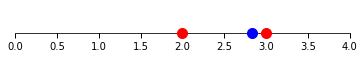
\includegraphics[scale=0.75]{lower_upper}
			\captionof{figure}{The lower and upper integer bounds for an arbitrary input.}
			\label{fig:lower_upper}
		\end{minipage}
	
		Vectors from the input coordinate to the two neighboring integer coordinates can then be calculated by subtracting each integer coordinate from the input \(x\) value. This gives a distance vector (which is one-dimensional in this case).
	
		\begin{lstlisting}[label={lst:dst}, language=Python, frame=none, caption={Calculating the distance.}, captionpos=b]
			d0 = x - x_min
			d1 = x - x_max
		\end{lstlisting}
	
		Now, both vectors necessary for the two influence values have been determined, giving a total of four vectors. The dot product of the distance vector and the respective gradient value can now be found. In the example below, the gradient values are being held in a one dimensional matrix of pseudo-random values, named \lstinline|lattice1d|
		
		\begin{lstlisting}[label={lst:influence}, language=Python, frame=none, caption={Calculating the influence values.}, captionpos=b]
			s = lattice1d[x_min] * d0
			t = lattice1d[x_max] * d1
		\end{lstlisting}
	
		Finally, these two values can be linearly interpolated with \(x - x_min\). This calculation is to put the x value into the interval of \([x_min, x_max]\).
		
		\begin{lstlisting}[label={lst:perlin_linear}, language=Python, frame=none, caption={Linear interpolation of influence values}, captionpos=b]
			x = x - x_min
			return lerp(s, t, x)
		\end{lstlisting}
	
		Iterating this function over the interval of \([0,10]\) results in the graph shown in \ref{fig:perlin_lin}. Note the jaggedness of the graph. This is the result of only using linear interpolation.
		
		\begin{minipage}{\textwidth}
			\centering
			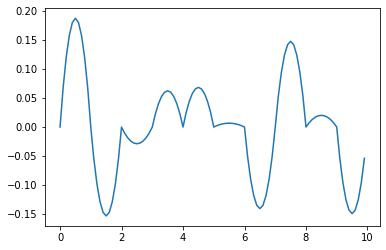
\includegraphics[scale=.5]{perlin_lin}
			\captionof{figure}{Example of Perlin noise using linear interpolation.}
			\label{fig:perlin_lin}
		\end{minipage}
	
		To smooth out the graph, a smoothing function, such as smoothstep interpolation can be applied to the input \(x\) values to make changes more gradual when approaching the integer coordinates. The suggested formula by Perlin for this interpolation was \(3t^2 - 2t^3\), but has since been superseded. One of the problems with the previous equation used was that the second derivative of the function, \textbf{6-12t} is not zero at either \textbf{t=0} or \textbf{t=1}, causing discontinuities in the noise. Some of the effects of this are shown in \autoref{fig:pnartifact}.
		
		\begin{minipage}{\textwidth}
			\centering
			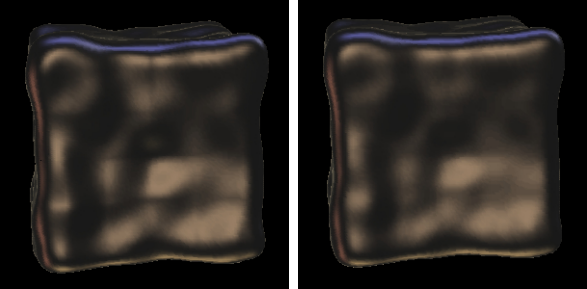
\includegraphics[scale=.5]{s-curve}
			\captionof{figure}{Removal of artifacting at t=0 and t=1 from revised interpolation function \cite{10.1145/566654.566636}}
			\label{fig:pnartifact}
		\end{minipage} 
		
		This led the improved equation. 
		
		\[t = 6t^5 - 15t^4 - 10t^3\]
		
		Putting it all together with smoothstep interpolation, Perlin noise can be implemented as such. 
		
		\begin{lstlisting}[label={lst:perlin1d}, language=Python, frame=none, caption={1D Perlin Noise}, captionpos=b]
			def perlin1d(x, lattice):
			
				x_min = int(x)
				x_max = x_min + 1
				
				xu = x - x_min
				xu = smoothstep(xu)
				
				d0 = x - x_min
				d1 = x - x_max
				
				# Influence values
				s = lattice[x_min] * d0
				t = lattice[x_max] * d1
				
				return lerp(s, t, xu)
			
			# Linear Interpolation
			def lerp(low, high, t):
				return low * (1-t) + high * t
			
			# Smoothstep
			def smoothstep(t):
				# 6t^5 - 15t^4 - 10t^3
				return t * t * t * (t * (t * 6 - 15) + 10)
		\end{lstlisting}
	
		This implementation results in noise such as the one depicted in \autoref{fig:perlin1d}.
		
		\begin{minipage}{\textwidth}
			\centering
			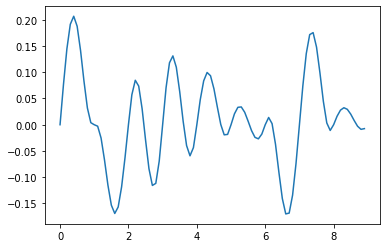
\includegraphics[scale=.5]{perlin1d}
			\captionof{figure}{One-dimensional Perlin noise.}
			\label{fig:perlin1d}
		\end{minipage} 
	
		\section{2-Dimensional}
		
		In two-dimensional Perlin noise, the associated lattice is a coordinate grid. The algorithm functions the same as one-dimensional Perlin noise, but instead of two surrounding points and working in a one-dimensional unit, two-dimensional Perlin noise works with four surrounding integer coordinate points, a unit square. Each of the corner points on the unit square now has a two dimensional gradient vector, holding the pseudo-randomly generated values. 
		
		\begin{minipage}{\textwidth}
			\centering
			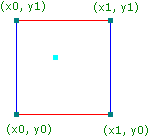
\includegraphics[scale=1.0]{cornergridpoints}
			\captionof{figure}{Arbitrary coordinate, surrounded by integer coordinate points (unit square) \cite{pn-math}.}
			\label{fig:cornergridpoints}
		\end{minipage} 
	
		Now, four influence values need to be calculated. Given a new two-dimensional coordinate point of \((x,y)\), the same operations must be taken. First, the minimum and maximum bounds must be found for both the \(x\) and \(y\), the same way they were found in one dimension. The combination of these four values results in the four corner points of the unit square surrounding the point of interest. The distance vectors are calculated the same way. 
		
		\begin{lstlisting}[label={lst:2d-dst}, language=Python, frame=none, caption={Calculating the distance for two-dimensions.}, captionpos=b]
			dx0 = x - x_min
			dx1 = x - x_max
			
			dy0 = y - y_min
			dy1 = y - y_max
		\end{lstlisting}
	
		\begin{minipage}{\textwidth}
			\centering
			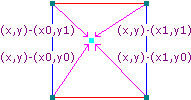
\includegraphics[scale=0.75]{2d_dist}
			\captionof{figure}{Example distance vector calculation \cite{pn-under}.}
			\label{fig:2d_dist}
		\end{minipage} 
	
		Then, the dot product of the distance vectors and their respective gradient vector is calculated. 
		
		\begin{lstlisting}[label={lst:2d-infl}, language=Python, frame=none, caption={Calculating the influence values for two-dimensions.}, captionpos=b]
			s = np.dot(lattice[x_min, y_min], [dx0, dy0])
			t = np.dot(lattice[x_max, y_min], [dx1, dy0])
			u = np.dot(lattice[x_min, y_max], [dx0, dy1])
			v = np.dot(lattice[x_max, y_max], [dx1, dy1])
		\end{lstlisting}
	
		Following this, the influence values must be interpolated. To do this, we can take three linear interpolations. 
		
		\begin{lstlisting}[label={lst:2d-interp}, language=Python, frame=none, caption={Calculating the interpolated final value.}, captionpos=b]
			v0 = lerp(s, t, xu)
			v1 = lerp(u, v, xu)
			
			return lerp(v0, v1, yu)
		\end{lstlisting}
	
		\begin{lstlisting}[label={lst:2d-perlin}, language=Python, frame=none, caption={Two-dimensional Perlin noise.}, captionpos=b]
			def perlin2d(x, y, lattice):
			
				x_min = int(x)
				x_max = x_min + 1
				
				y_min = int(y)
				y_max = y_min + 1
				
				xu = x - x_min
				xu = smoothstep(xu)
				
				yu = y - y_min
				yu = smoothstep(yu)
				
				dx0 = x - x_min
				dx1 = x - x_max
				
				dy0 = y - y_min
				dy1 = y - y_max
				
				# Influence values
				s = np.dot(lattice[x_min, y_min], [dx0, dy0])
				t = np.dot(lattice[x_max, y_min], [dx1, dy0])
				u = np.dot(lattice[x_min, y_max], [dx0, dy1])
				v = np.dot(lattice[x_max, y_max], [dx1, dy1])
				
				v0 = lerp(s, t, xu)
				v1 = lerp(u, v, xu)
				
				return lerp(v0, v1, yu)
			
			# Linear Interpolation
			def lerp(low, high, t):
				return low * (1-t) + high * t
			
			# Smoothstep
			def smoothstep(t):
				# 6t^5 - 15t^4 - 10t^3
				return t * t * t * (t * (t * 6 - 15) + 10)
		\end{lstlisting}
	
		This will result in an image such as \autoref{fig:lect14-perlin}, where the output values are interpreted as grayscale color values. 
		
		\begin{minipage}{\textwidth}
			\centering
			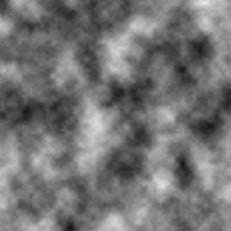
\includegraphics[scale=1.0]{lect14-perlin}
			\captionof{figure}{Two-dimensional Perlin noise \cite{noise-ex}.}
			\label{fig:lect14-perlin}
		\end{minipage} 
		
		\section{3-Dimensional}
		
		Three dimensional Perlin noise follows the same pattern. In one dimension, calculations were required for each of the two points surrounding the point in question. In two dimensions, calculations were required for the four points of the unit square. In three, this becomes eight for the unit cube. From this, Perlin noise's runtime scaling can be determined - \(O(2^k)\), where \(k = dimensionality\). 
		
		\section{N-Dimensional}
		
		While Perlin noise saw great success, it was succeeded by algorithms such as Simplex noise, designed to alleviate some of the problems with Perlin noise. This included the computational complexity and the artifacting in the noise created. The artifacting in the noise appears from the necessity for the gradients to pass through zero at the integer coordinates of the lattice. This causes unavoidable artifacting in the noise. In addition, while Perlin noise's computational complexity is acceptable when in three-dimensional space and lower, it suffers greatly from increasing the dimensionality further. Beyond three-dimensional space and its unit cubes, four-dimensional space and beyond's unit cube equivalent is known as a hypercube. The number of corners a hypercube has is \(O(2^k)\), where \(k = dimensionality\). This runtime scaling makes higher dimensions incredibly hard to calculate. 
		
		Simplex noise was designed to address some of the limitations of the original Perlin noise. Since the original implementation of Perlin noise was constrained by the lattice gradient function creating directional artifacts, one of the goals of Simplex noise was to overcome this limitation. In addition, Simplex noise has lower computational complexity -- O(k\textsuperscript{2}) instead of O(2\textsuperscript{k})\cite{sheet-simplex}. Other benefits includes the capability to scale to higher dimensions, a well-defined and continuous gradient, as well as simpler implementation. Instead of the lattice gradients that Perlin noise works on, and that give Perlin noise its computational complexity, Simplex noise works based on simplex grids for which it was named after. This involves choosing the simplest, repeatable shape to fill a N-dimensional space. Another definition of a n-simplex would be it being the smallest figure that contains \(n+1\) given points in n-dimensional space, while not lying in the space of a lower dimension. In one dimension, this works by choosing repeating line segments, similarly to Perlin noise. In two dimensions, this becomes an equilateral triangle, contrary to the unit square of Perlin noise. In three dimensions, this becomes a trianglular pyramid, also known as a tetrahedron. From four dimensions and onward, this simplex becomes increasingly difficult to visualize. However, there is a pattern in the drawability of simplexes, by creating a new point and connecting it to all previously existing points.
		
		\begin{minipage}{\textwidth}
			\centering
			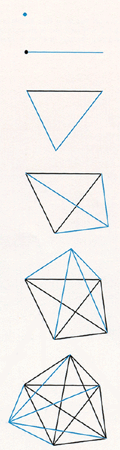
\includegraphics[scale=.75]{six simplexes}
			\captionof{figure}{The first six simplexes \cite{higher-dim-simplexes}}
			\label{fig:fig2}
		\end{minipage}
		
		The relative simplicity of the simplex shape in having as few corners as possible makes it a lot easier to interpolate values in the interior of the shape, relative to the hypercubes used in the original Perlin noise.
		
		In the original Perlin noise function, derivatives were used to compute the gradation between the points. This creates a large increase in computational complexity based on dimensionality. Simplex noise instead uses the summation of kernel values to determine the point's value. To generate the Simplex noise, the value for any point in space must be determined. In two dimensional space, this means skewing the coordinate space along the main diagonal, transforming the squashed equilateral triangles into right-angle isosceles triangles. From there, determining the location is made more simple, as just the integer part of the coordinates is needed for each dimension. Beyond two dimensions, the visualization becomes more difficult, but the steps remain the same.  
		
		\begin{minipage}{\textwidth}
			\centering
			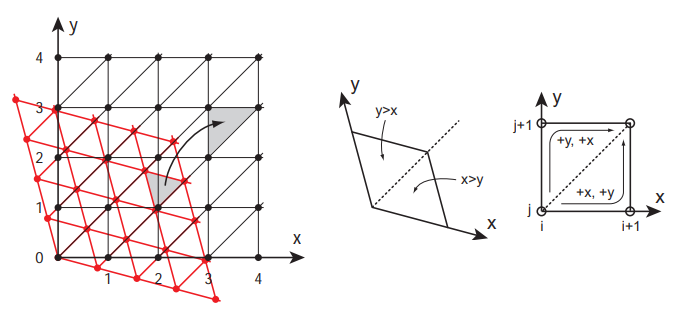
\includegraphics[scale=.5]{skewed grid}
			\captionof{figure}{Skewing in two-dimensional space and determining the cell containing a point. \cite{simplex-demyst}}
			\label{fig:fig9}
		\end{minipage}
		
		The traversal scheme for a two-dimensional simplex is built around this triangular shape. If the x and y coordinates are known, then all that is needed is to determine which of the two simplices the point lies in. If x > y, the corners become (0,0), (1,0) and (1,1), else the corners are (0,0), (0,1) and (1,1). To traverse this, only one step in the x and one step in the y is needed, but in a different order for each of the simplices. This can then be generalized to any arbitrary amount of N dimensions \cite{simplex-demyst}. While Perlin noise has many advantages over the classical Perlin noise, it has a different visual characteristic, making it difficult to directly replace or compare the two. 
		
		\begin{minipage}{\textwidth}
			\centering
			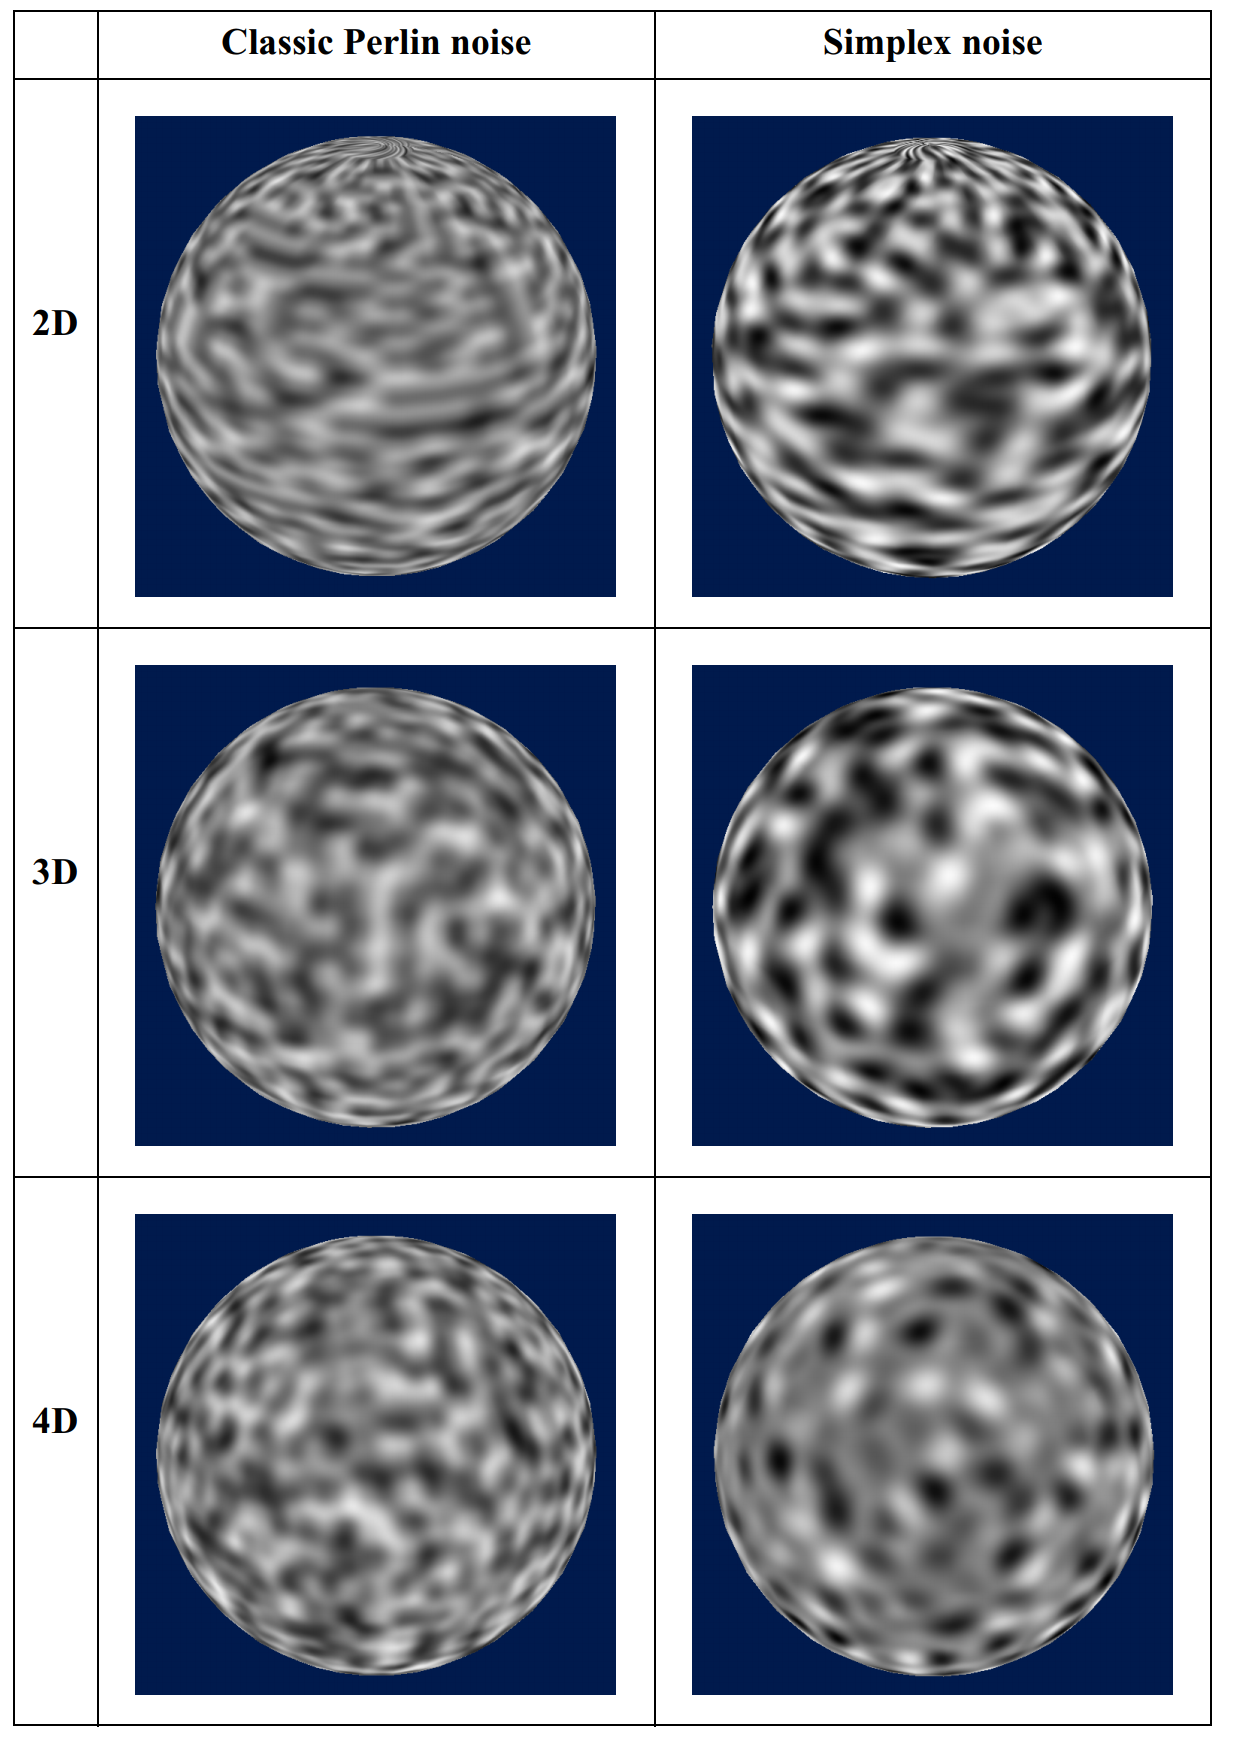
\includegraphics[scale=.2]{perlin vs simplex}
			\captionof{figure}{A comparison of Perlin and Simplex noise \cite{simplex-demyst}}
			\label{fig:fig4}
		\end{minipage}
		
		However, with additional modification using multiple layers or octaves, Simplex noise will run much more computationally efficiently, as well as replicating the visual quirks of Perlin noise.
		
		\section{Modifications}
		To add more diversity, and to increase the range of values given by Perlin noise, octaves can be added. The term octave is borrowed from music, where a musical tone that is one octave higher than the previous tone has double the frequency. In Perlin noise, this frequency relationship is typically preserved, with increasing octaves of Perlin noise having double the frequency. In simpler terms, the frequency of Perlin noise determines the number of steps taken in total. Some additional terms for octaves in Perlin noise include amplitude, which refers to the range of output values that are possible, as well as the persistence, which refers to the influence that the octave has. Adding octaves together will increase detail, but scales runtime linearly \cite{pn-under}. 
		
		\subsection{Hashing} \label{subsec:hashing}
		Perlin's improved noise implements a hash function instead of using a true random number table \cite{improv-noise}. This both serves as an efficient storage method, as each random number needed can be algorithmically determined from the coordinate point, as well as allowing for memory constraints to be lowered, due to the need for just a hashing function. Perlin's hashing function consists of the set of integers in \([0, 255]\), ordered randomly, as shown in \autoref{lst:hashtable}. 
		
		\begin{lstlisting}[label={lst:hashtable}, language=Python, frame=none, caption={Perlin's hashing table}, captionpos=b]
			p = [ 151,160,137,91,90,15,
			131,13,201,95,96,53,194,233,7,225,140,36,103,30,69,142,8,99,37,240,21,10,23,
			190, 6,148,247,120,234,75,0,26,197,62,94,252,219,203,117,35,11,32,57,177,33,
			88,237,149,56,87,174,20,125,136,171,168, 68,175,74,165,71,134,139,48,27,166,
			77,146,158,231,83,111,229,122,60,211,133,230,220,105,92,41,55,46,245,40,244,
			102,143,54, 65,25,63,161, 1,216,80,73,209,76,132,187,208, 89,18,169,200,196,
			135,130,116,188,159,86,164,100,109,198,173,186, 3,64,52,217,226,250,124,123,
			5,202,38,147,118,126,255,82,85,212,207,206,59,227,47,16,58,17,182,189,28,42,
			223,183,170,213,119,248,152, 2,44,154,163, 70,221,153,101,155,167, 43,172,9,
			129,22,39,253, 19,98,108,110,79,113,224,232,178,185, 112,104,218,246,97,228,
			251,34,242,193,238,210,144,12,191,179,162,241, 81,51,145,235,249,14,239,107,
			49,192,214, 31,181,199,106,157,184, 84,204,176,115,121,50,45,127, 4,150,254,
			138,236,205,93,222,114,67,29,24,72,243,141,128,195,78,66,215,61,156,180
			]
			
			
		\end{lstlisting}
	
		\begin{lstlisting}[language=Python, frame=none, caption={Unit cube's corner minimum values}, captionpos=b]
			...
			x_min = int(x)
			x_max = x_min + 1
			
			y_min = int(y)
			y_max = y_min + 1
			
			z_min = int(z)
			z_max = z_min + 1
			...
		\end{lstlisting}
		
		To calculate the random value needed for a given \((x,y,z)\) point, eight values must be calculated, for the unit cube surrounding the point. First, the value of the minimum and the maximum bound of the unit cube in the x dimension must be hashed. 
		
		\begin{lstlisting}[label={lst:hashx}, language=Python, frame=none]
			A = p[x_min]
			B = p[x_max]
		\end{lstlisting}
		
		Then, the value of the minimum and the maximum bound of the unit cube in the y dimension will each be added to each of these hash values, resulting in four total values. 
		
		\begin{lstlisting}[label={lst:hashx}, language=Python, frame=none]
			AA = p[A + y_min]
			BA = p[B + y_min]
			
			AB = p[A + y_max]
			BB = p[B + y_max]
		\end{lstlisting}
	
		Lastly, the  minimum and the maximum bound of the unit cube in the z dimension will each be added to each of these hash values, resulting in eight total values -- one for each corner of the unit cube. 
		
		\begin{lstlisting}[label={lst:hashx}, language=Python, frame=none]
			AAA = p[AA + z_min]
			AAB = p[AA + z_max]
			
			BAA = p[BA + z_min]
			BAB = p[BA + z_max]
			
			ABA = p[AB + z_min]
			ABB = p[AB + z_max]
			
			BBA = p[BB + z_min]
			BBB = p[BB + z_max]
		\end{lstlisting}
		
	\vspace{10pt}
	\let\clearpage\relax
	\chapter{Data Structures} \label{chap:data_structures}
	
		\section{Chunking}
			PGC has the advantage of being able to be recreated through the use of the correct seed and algorithm. For example, to efficiently store the topological data generated from a procedural algorithm, the topological data can be broken into smaller pieces. These pieces may be known as chunks \cite{tiling}. This compartmentalizes the procedural algorithm. By chunking the data necessary to generate, it is not required to generate every single number in the lattice at a time, to determine the values of new edge points. Instead, only the values in the local chunk will be determined. In cases of extremely large-scale topography, where the user may not need or may not see the entire map at the same time, chunking allows for the algorithm to still run. For Perlin noise with multiple octaves and three-dimensional complexity, while memory is not as much of a concern as it was in the past, this helps to alleviate some of the computational strain that can be caused. 
	
		\section{Height Maps}
			
			Another common method of storing topological data is through the use of height maps. 
			
			\begin{minipage}{\textwidth}
				\centering
				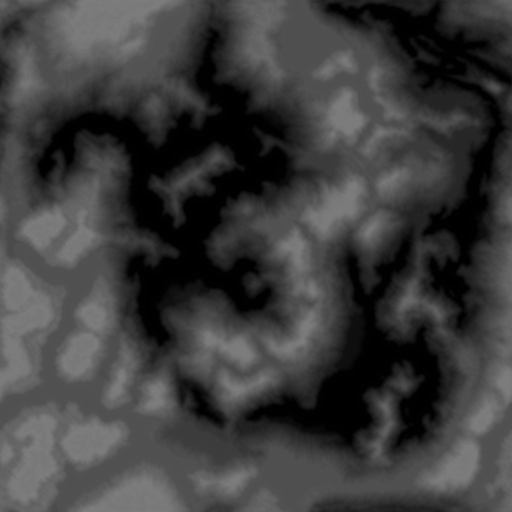
\includegraphics[scale=.4]{D10}
				\captionof{figure}{An example of a height map. \cite{voxel-space}}
				\label{fig:height-map}
			\end{minipage}
			
			The use of height maps is related to the development of some image based rendering and displaying procedural content. A height map works by storing a single height value at each \[(x,y)\] coordinate. Height maps work similarly to topological maps, with an example of the latter shown in \autoref{fig:top-map}.
			
			\begin{minipage}{\textwidth}
				\centering
				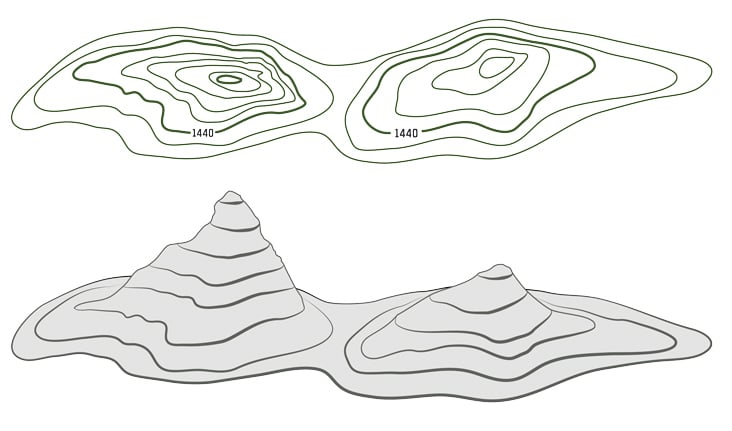
\includegraphics[scale=.4]{top-map}
				\captionof{figure}{A topological map is shown, with a corresponding three-dimensional representation of the map data below. \cite{top-map}}
				\label{fig:top-map}
			\end{minipage} 
		
			Height maps can be combined with a color map of the same dimensions, in order to map colors to each of the height locations. This effect can be seen in voxel space rendering, shown in \ref{sec:imagebasedmethods} In terms of generating geological formations for landmarking a terrain, height maps add additional limitations on the possibilities. Height maps are unable to store multiple data values at each point, without significant complexity in interpreting the resultant data. This makes the generation of overhangs, arches, or any feature with protruding structures, difficult without additional data storage for these exceptions. A possible solution for this issue includes the storage of overhangs or similar features separately.
		
	\vspace{10pt}
	\let\clearpage\relax
	\chapter{Rendering Methods}
	
		Representing the data generated procedurally is another task with a variety of solutions. Some of these methods include image-based rendering, polygons, and voxels. One common, simplistic way to represent the data generated is to use ASCII characters, or other types of two-dimensional data such as colored pixels to convey the scene that is being represented. In the case of Dwarf Fortress, the use of ASCII symbols is used to represent the elements within the game, shown in \autoref{fig:asciidf}. The interpretation of procedurally generated data will be expanded upon in \autopageref{chap:interpret}
		
		\begin{minipage}{\textwidth}
			\centering
			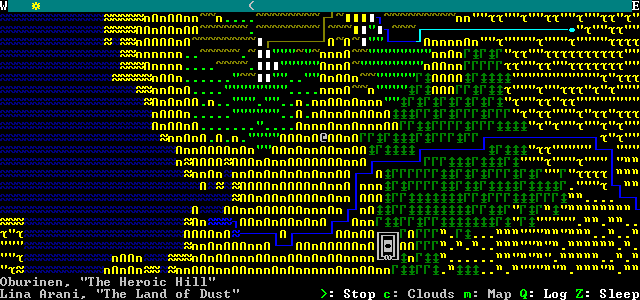
\includegraphics[scale=.5]{dwarf_fortress}
			\captionof{figure}{ASCII representation of PGC. \cite{df-dev}}
			\label{fig:asciidf}
		\end{minipage}
	
		\section{Image Based Rendering} \label{sec:imagebasedmethods}
		
		Image based rendering work by rendering based on the screen resolution of the output and the resolution of the input, rather than storing geometric positions. One example of image based rendering is the voxel space rendering system. The voxel space rendering system uses voxel raster graphics to display three-dimensional geometry with low memory and processing requirements. This was developed in the early 90's, involving a height and color map to position the pixels on the screen. While voxel space rendering was not historically used with noise generating algorithms, the rendering system fits the requirements for the use of procedural algorithms such as two-dimensional Perlin noise. By using Perlin noise, the height and color maps can be generated at run-time instead of being created beforehand. An example of this is shown in \autoref{fig:pnvs}. At the time, displaying complex height-maps in three-dimensions was difficult computationally, and voxel space rendering served as a workaround. 
		
		\begin{minipage}{\textwidth}
			\centering
			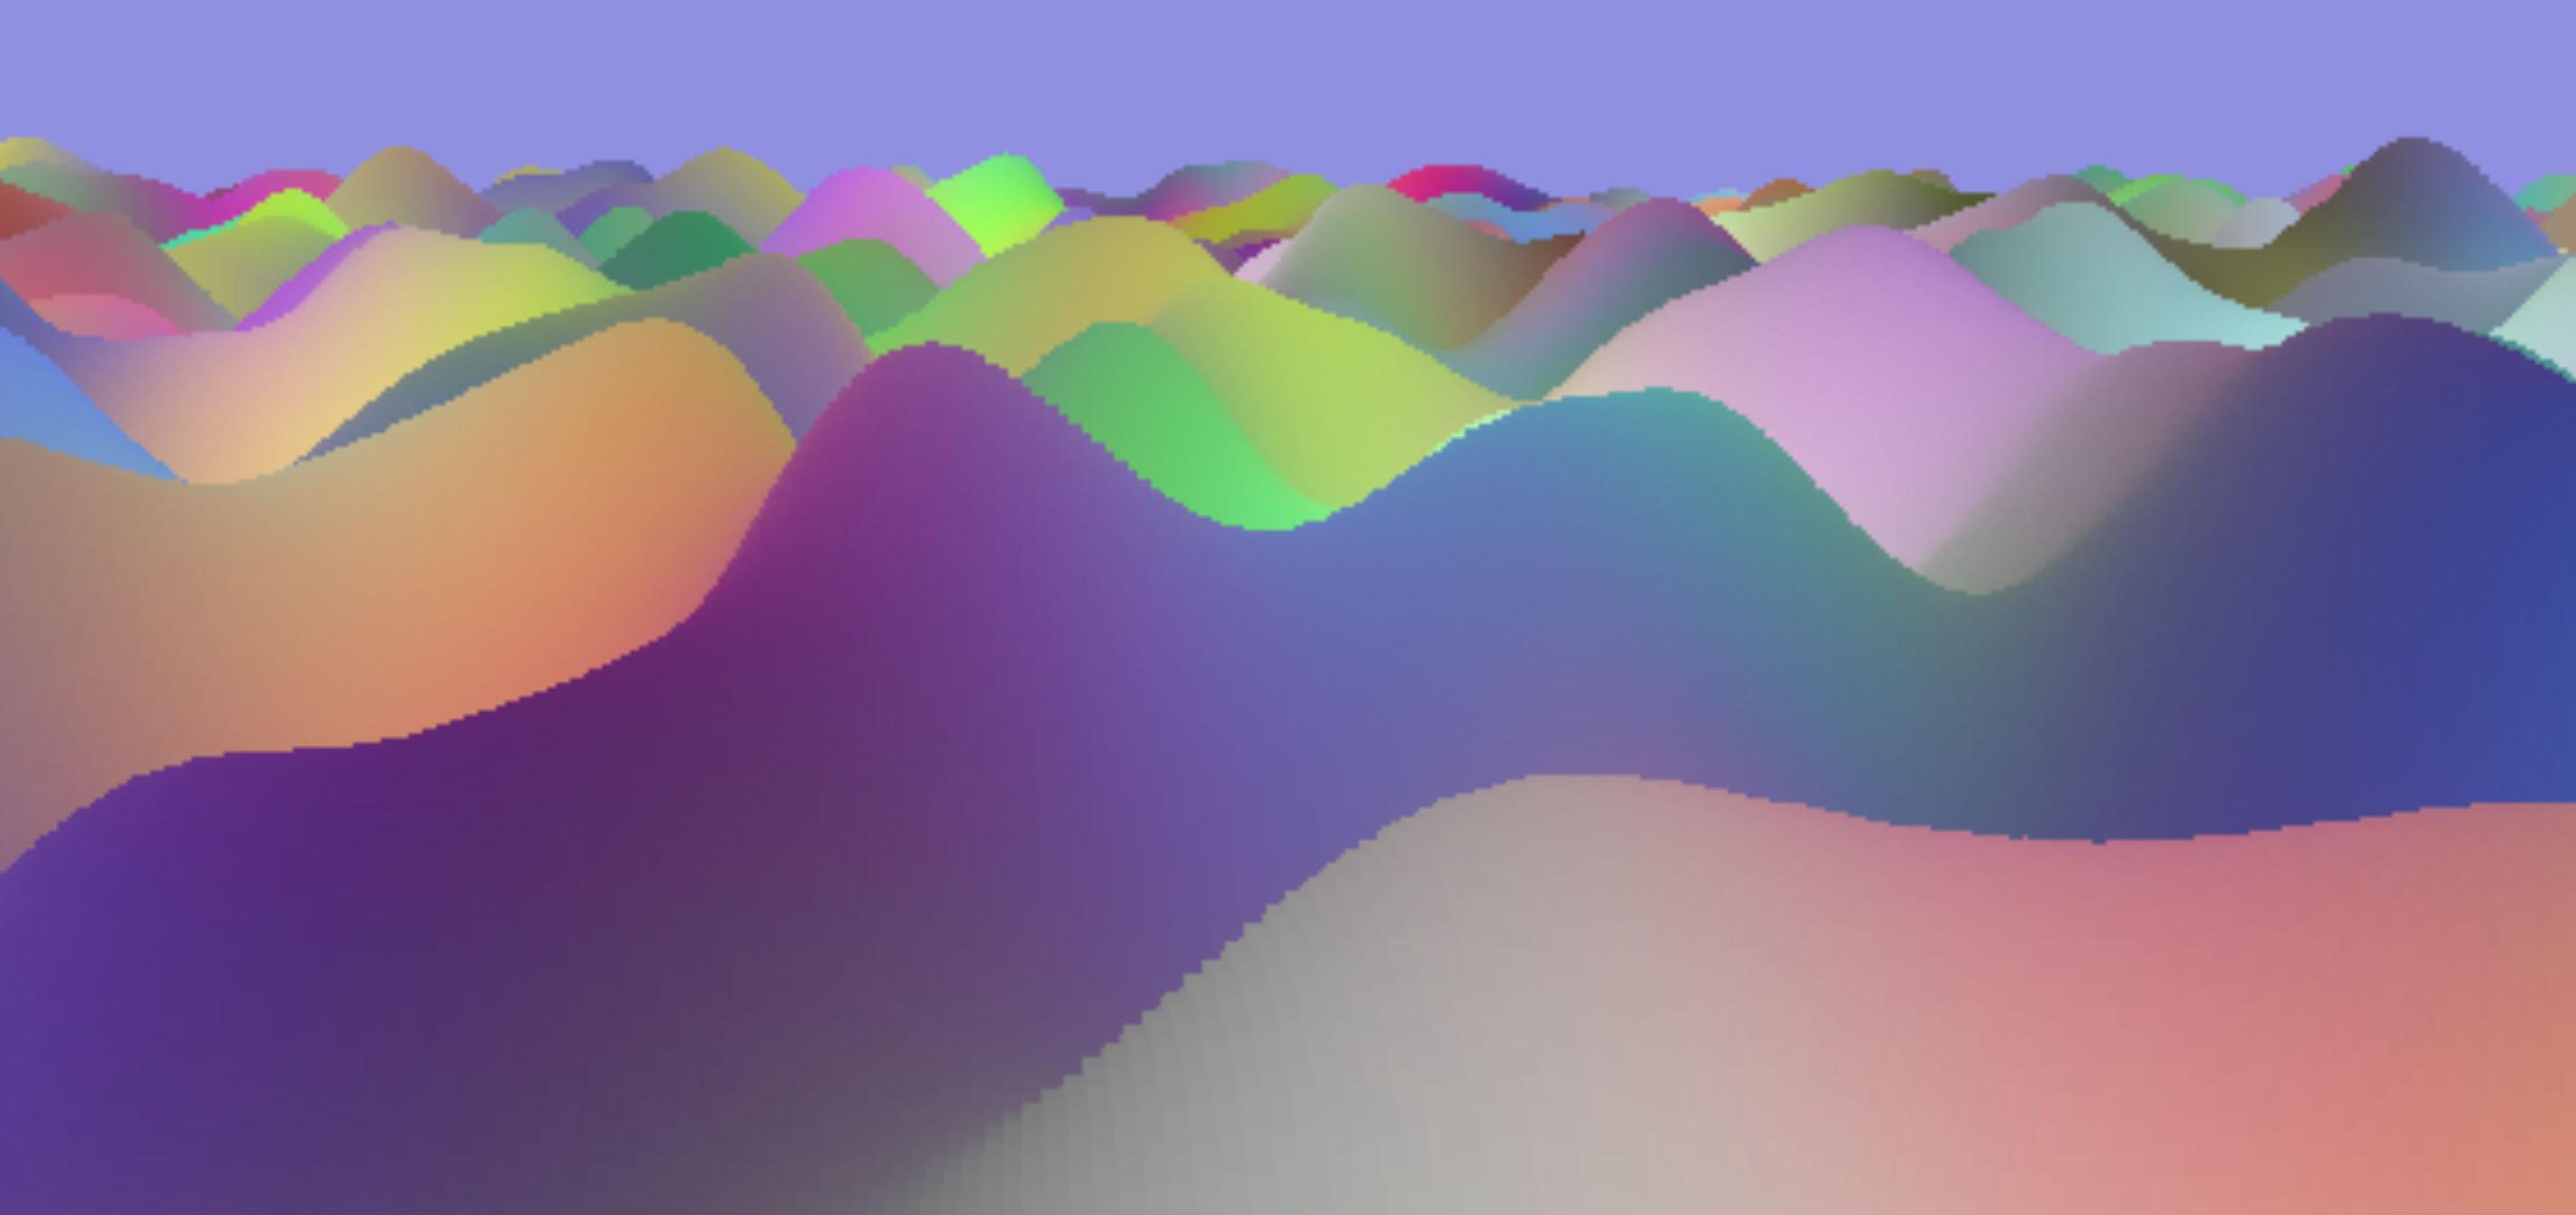
\includegraphics[scale=.15]{proc-voxel}
			\captionof{figure}{Rendering using the Voxel Space engine with a height and color map generated by Perlin noise.}
			\label{fig:pnvs}
		\end{minipage}
		
		The voxel space rendering engine originally utilized a pre-made height and color map to render from. This, combined with a tiling effect and knowledge of the field-of-view of the user's position allowed for a simplified three-dimensional rendering system. Starting from the furthest position to guarantee occlusion, a line on the map is determined in the triangular field of view. This is scaled with perspective projection, and a vertical line is drawn at every point on the screen from the section of the color map. The height of the vertical line is determined from the height drawn from the two-dimensional height map. Then, this is repeated until the entire field-of-view is drawn. This occlusion can be seen in \autoref{fig:vs-raster}. 
		
		\begin{minipage}{\textwidth}
			\centering
			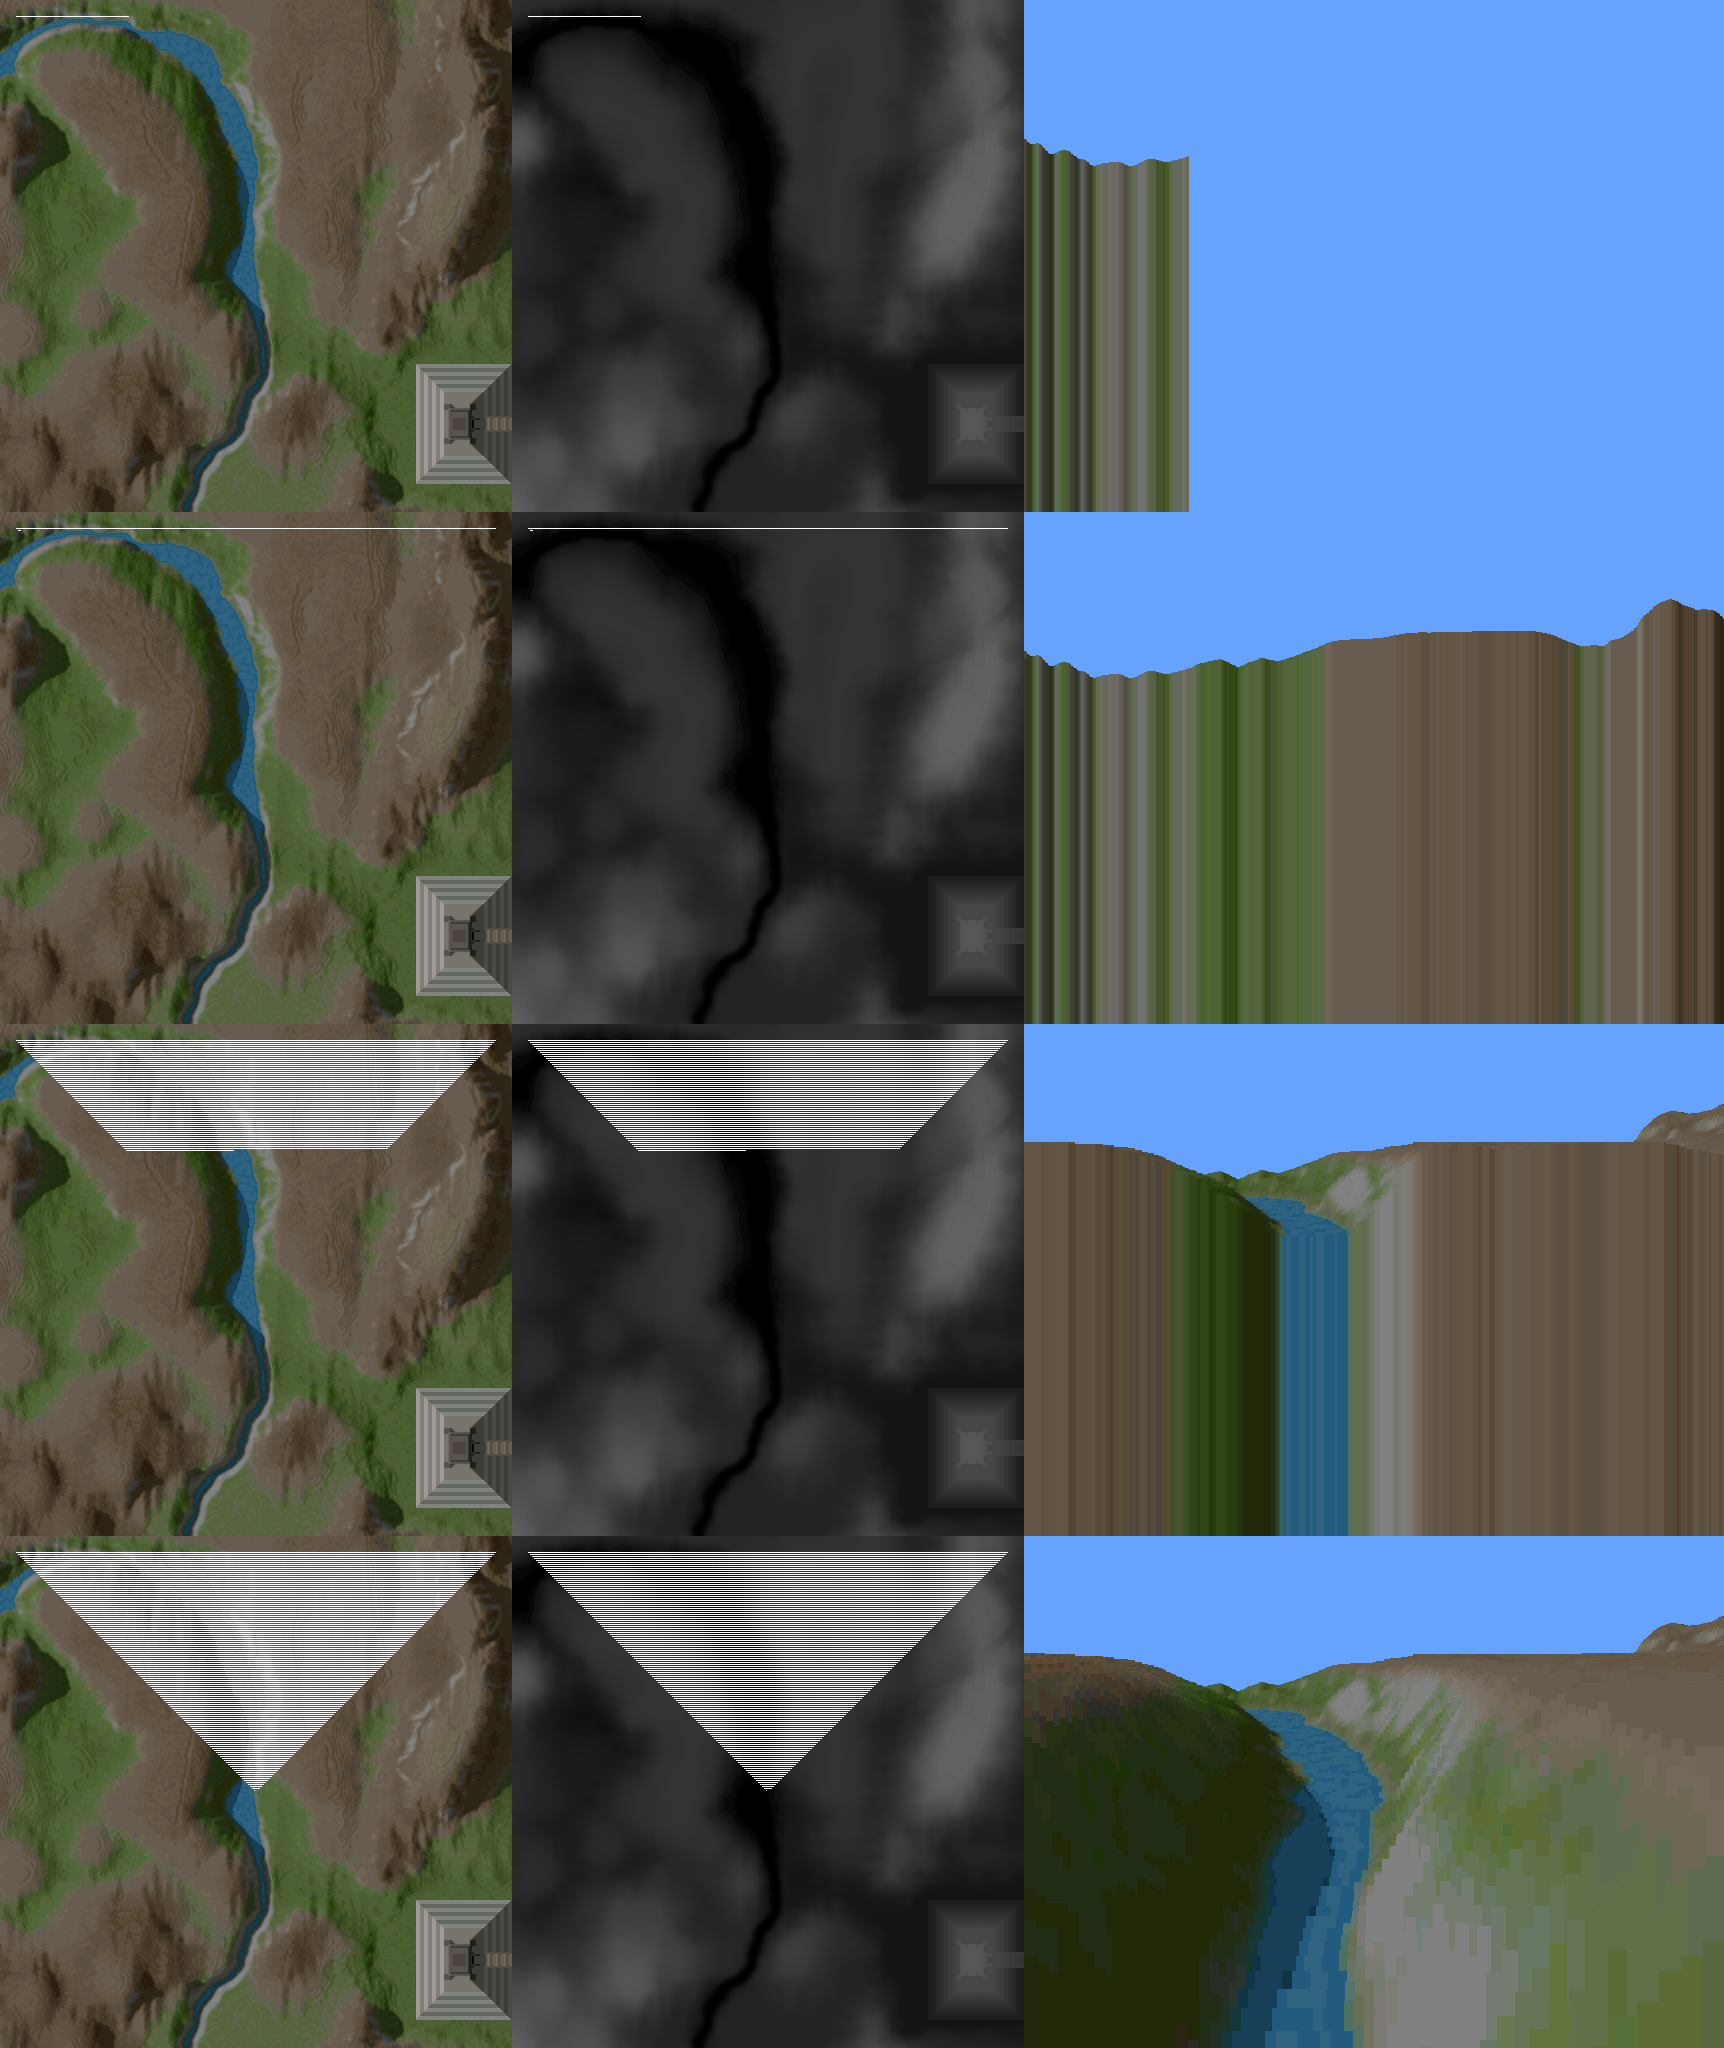
\includegraphics[scale=.2]{line-by-line}
			\captionof{figure}{Basic rasterization of the Voxel Space engine \cite{voxel-space}.}
			\label{fig:vs-raster}
		\end{minipage}
	
		This can be optimized with drawing from front-to-back with the addition of a y-buffer to determine the highest y position to draw. In this case, the y-buffer holds the highest y position, guaranteeing that the closest regions of the height map are displayed properly. However, the voxel-space rendering system has a downside of having fewer pixels to determine the colors and heights of closer landmasses. This creates a pixellated effect for the foreground, while the background is rendered in higher detail. This pixellation and rendering system can be seen in more detail in \autoref{fig:vs-patent}. 
		 
		\begin{minipage}{\textwidth}
		 	\centering
		 	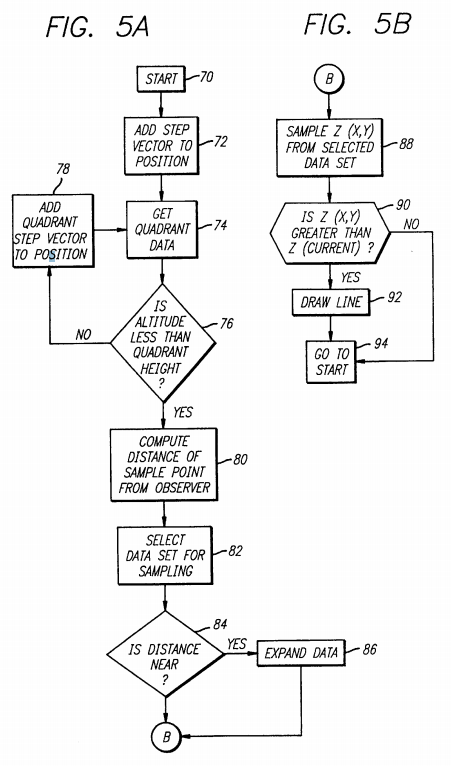
\includegraphics[scale=0.5]{US6020893A}
		 	\captionof{figure}{US Patent 6 020 893 \cite{US6020893}.}
		 	\label{fig:vs-patent}
		\end{minipage}
		
		This weakness can be mitigated in some effect by having multiple heightmaps of differing detail to draw from. This would mitigate some of the advantage of voxel space rendering in increasing the rendering time and processing required for the algorithm. In addition to the weakness in rendering closer objects, height maps are also unable to render more complex geological formations, such as caves, archways or overhangs. Later iterations of the voxel space rendering engine worked around some of these limitations by introducing rendering of both polygons and voxels. Another possible workaround to the low resolution of the voxel space rendering system would be using procedurally generated noise as the platform for creating height maps. By creating the height map dynamically from noise, the memory used for storing the program overall would be smaller, and the resolution would not be constrained, as for areas closer to the camera, the interpolation between the points of the noise map would just be decreased. 	
	
		\section{Polygononal Meshes}
	
		Using a polygonal mesh to represent an object is a common way to representing objects on a computer. A polygon is a planar shape, defined by connecting a series of vertices. A polygon mesh is composed of polygons, and is defined by three parts.
		
		\begin{center}
			\begin{tabular}{ l l } 
				V & a set of vertices (points in space)\\ 
				$E {\subset} (V x V)$ & a set of edges (line segments)\\ 
				$F {\subset} E^{\ast}$  & a set of faces \\
			\end{tabular}
		\end{center}
		% https://www.classes.cs.uchicago.edu/archive/2015/fall/23700-1/docs/mesh-notes.pdf
	
		These parts allow for the definition of a shape, composed of polygons. Triangles are the default polygon for use in polygonal meshes, the vertices composing the face of a triangle all have to occupy the same plane \cite{polygon}. By connecting the faces of multiple triangles, it is possible to assemble more complex shapes. For example, two right angle triangles connected along the hypotenuse edge will create a square, then six of these squares can be connected to form a cube. While this takes twelve triangles to represent, there are only eight unique vertices that need their position defined. An example of a polygonal mesh is shown in \autoref{fig:utah-teapot}.
		
		\begin{minipage}{\textwidth}
			\centering
			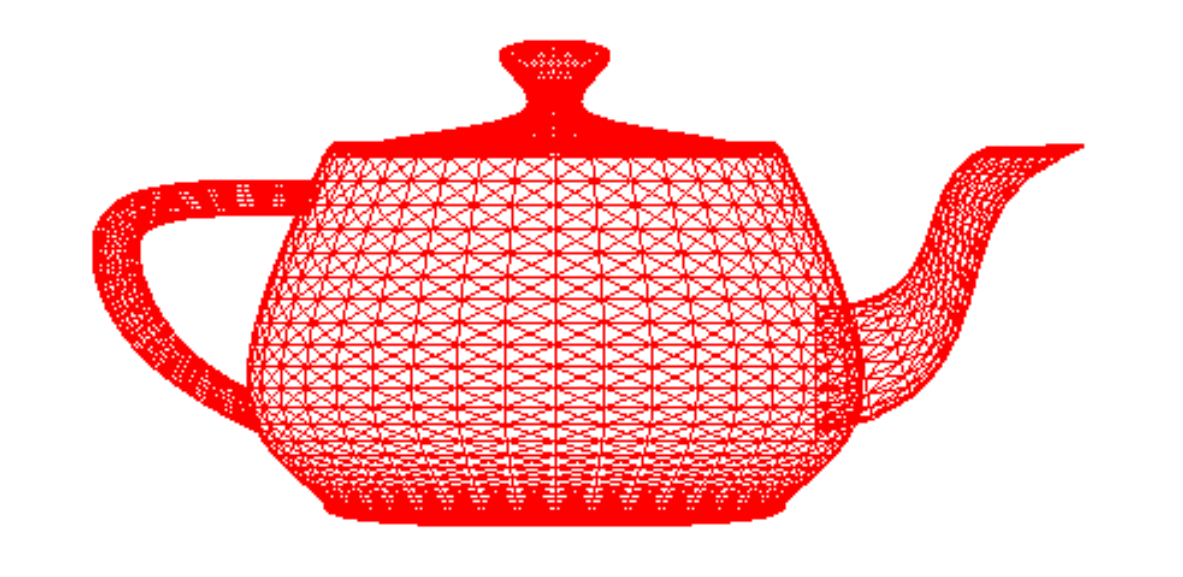
\includegraphics[scale=0.3]{utah-teapot}
			\captionof{figure}{A polygonal mesh of the Utah Teapot \cite{utah-teapot}.}
			\label{fig:utah-teapot}
		\end{minipage}	
		
		\section{Voxels}
	
		In contrast to polygons, voxels represent a volume element in space. Voxels act as a three-dimensional version of a pixel in space. While voxels are typically contained within a cubic cell in three-dimensions, they are not limited to this shape, and can have any number of shapes. These indivudual elements contain its position in space and another parameter or set of parameters, ranging from the color to the material to the texture data, among other possibilities. This allows for easier computation of the absence of terrain data, such as in caves or polygons. In terms of creating a cave, the points in space representing the cave just need to be removed, in contrast to the mapping required to store the vertices in space. 
		
		While the success of Minecraft has made it the atypical example of procedural generation rendered using voxels, the representation of voxels as cubes stacked in space is not accurate to the greater definition of the voxels being volume elements in space. Minecraft does use a voxel system to store the points in space as data, indexed by an YZX system for compression \cite{minecraft-voxel}. However, Minecraft's rendering system is based around a polygon system to display the individual blocks. 
		
		\label{pt:marching_cubes}
		An example of a structure of representing voxel data is through the marching cubes algorithm. Each voxel (cube) in marching cubes is defined by the pixel values at the corners of the cube. These eight pixel values each contribute a single value, also known as a density value, with negative values indicating that the point is in empty space, and positive values indicating that the point is inside of solid terrain. A density value of 0, at the boundary of positive and negative, indicates the surface of the terrain. Along this surface is where the polygonal mesh is constructed \cite{marching-cubes}. At any voxel area contained within the eight points, the marching cubes algorithm allows generation of the correct polygons, outputting from zero to five polygons.
		
		To generate the polygons within the cell, the density values must be determined. The set of all corner vertices can be denoted as \(V = {v0,v1,v2,v3,v4,v5,v6,v7}\), where a positive density sets the vertex's bit to one, and a negative density sets the value to zero. 

		\begin{minipage}{\textwidth}
			\centering
			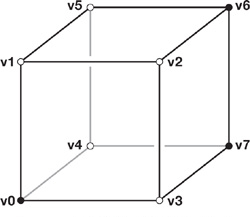
\includegraphics[scale=0.75]{01fig03}
			\captionof{figure}{A single voxel with example density values at the eight corner vertices \cite{marching-cubes}.}
			\label{fig:marching-cube}
		\end{minipage}
	
		\begin{center}
			\begin{tabular}{ l l } 
				\begin{tabular}{ l l }
					Case & = \\
				     	 & = \\
				     	 & = \\
				\end{tabular} 
				&
				\begin{tabular}{ r r r r r r r r }
					{ } v7$\vert$&v6$\vert$&v5$\vert$&v4$\vert$&v3$\vert$&v2$\vert$&v1$\vert$&v0\\
					{ } 1 $\vert$&1$\vert$&0$\vert$&0$\vert$&0$\vert$&0$\vert$&0$\vert$&1\\
					193&&&&&&&
				\end{tabular}
			\end{tabular}
		\end{center}
	
		These bit values can be concatenated with a bitwise OR operation to produce a single byte, in the range of 0-255. Two of these cases end up being trivial -- the concatenated value is 0 or 255, all the points are either inside of a solid terrain, or are in empty space. For the remaining configurations, there are only 14 unique combinations (shown in \autoref{fig:01fig04}) of the remaining 254 possibilities. This allows for the use of a look-up table to generate the polygons \cite{marching-cubes-paul}. 
		
		\begin{minipage}{\textwidth}
			\centering
			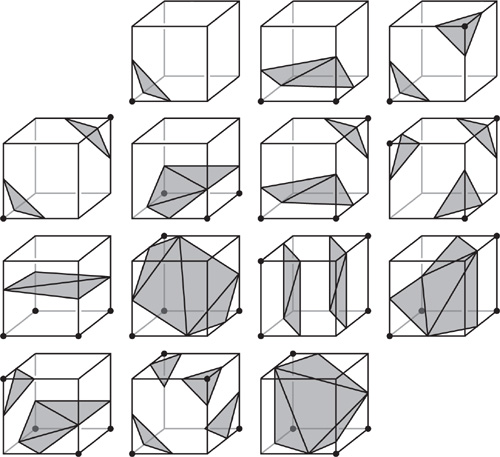
\includegraphics[scale=0.75]{01fig04}
			\captionof{figure}{A single voxel with example density values at the eight corner vertices \cite{marching-cubes}.}
			\label{fig:01fig04}
		\end{minipage}
	
		The placements of the vertices of each of these figures is determined by the density values for each of the corner points, by interpolating the value between these values.
		
	\vspace{10pt}
	\let\clearpage\relax
	\chapter{Interpretation} \label{chap:interpret}
		
		Procedural algorithms only generate a set of values. In order to transform these values into PGC, it must be interpreted into the desired outcome. Ultimately, this is a very subjective task, but this paper will cover three possible examples of interpretation. 
		
		A tileset is a two-dimensional grid interpretation of the display. This grid is uniform. One method of interpreting data is to interpret the values given from procedural generation into a tileset. This tileset approach can be seen in the example of Dwarf Fortress, given above. For example, in Dwarf Fortress, there are 256 possible outputs. Each of these possible outputs has an associated ASCII character, or an associated square image to serve as the interpreted output. 
		
		\begin{minipage}{\textwidth}
			\centering
			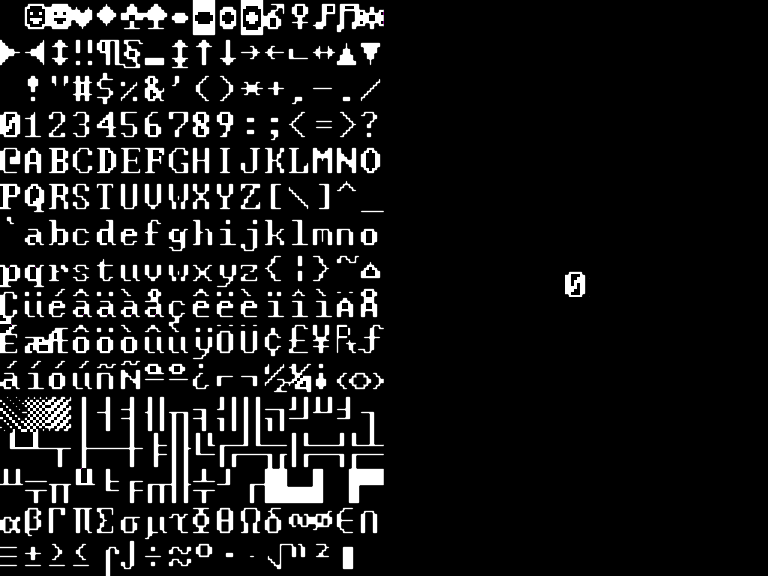
\includegraphics[scale=0.3]{Curses_1920x900}
			\captionof{figure}{A tileset grid pictured on the left half, with one singular 24x36 pixel tile on the right\cite{df-tileset}.}
			\label{fig:Curses_1920x900}
		\end{minipage}
	
		Tilesets work efficiently for rendering, and allow for complete control over the PGC, as every single possible output is individually controlled by the user. A single tile does not need to correspond to a single procedural value. For example, any procedurally generated value in the range of \([0,3]\) could be interpreted as one tile. 
		
		Another form of interpretation is associated with storage as well. This involves a heightmap, where the procedurally generated value is taken as a height value. These heightmaps can be rendered in a variety of ways, including using image-based rendering, polygons, or voxels. In \autoref{fig:terrain_mesh}, a heightmap was generated, then another algorithm was used to connect the different vertices together to create a polygonal mesh. 
		
		\begin{minipage}{\textwidth}
			\centering
			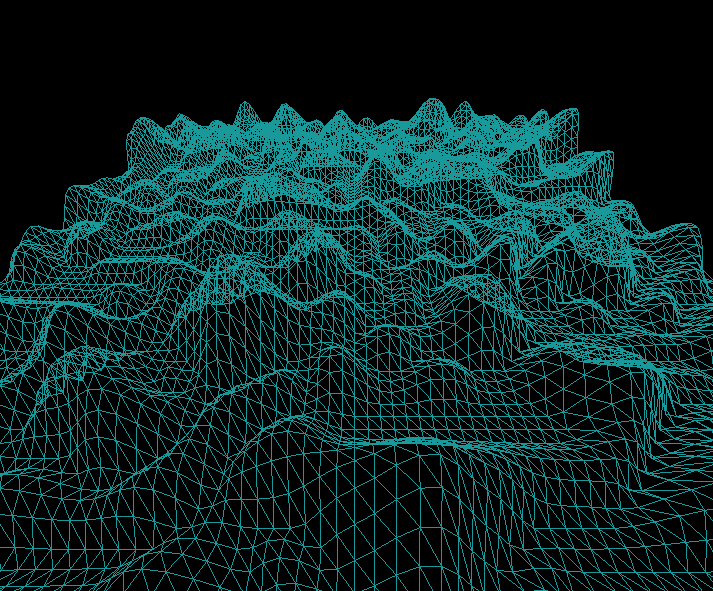
\includegraphics[scale=0.3]{terrain_mesh}
			\captionof{figure}{A heightmap mesh\cite{terrain_mesh}.}
			\label{fig:terrain_mesh}
		\end{minipage}
	
		The last interpretation of data that will be covered here is the interpretation of the procedural values as density values. This particular interpretation is what is used in the Marching Cubes algorithm (see \autoref{pt:marching_cubes}). 
		
		\begin{minipage}{\textwidth}
			\centering
			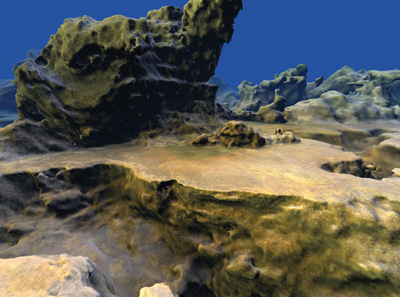
\includegraphics[scale=1.0]{marching}
			\captionof{figure}{Terrain created using the Marching Cubes algorithm\cite{marching-cubes}.}
			\label{fig:marching}
		\end{minipage}
	
		A texture is an image or color applied to the surface of a three-dimensional model. For the data created from heightmaps or Marching Cubes, there are also a number of ways to texture this topographical data. One example is similar to the tileset interpretation of procedural data -- just interpret a value, or range of values, as a single color. This often works well for heightmaps, as lower regions can be colored darker, or shaded with water, while higher regions can replicate snowy mountaintops. Another option is triplanar mapping, which blends three textures to create the least stretched image \cite{triplanar, marching-cubes}.  
		
	\vspace{10pt}
	\let\clearpage\relax
	\chapter{Development}
		
		\section{Fractals}
		Brownian motion was one of the starting points for procedural algorithms, used to describe the random motion of particles within water. Robert Brown first described this natural phenomenon in 1827. The stochastic process behind Brownian motion was later mapped into an algorithm almost a century later, a method called the Wiener process \cite{inbook}. A standard Wiener process on the interval \([0,T]\) is a random variable \(W(t)\), where \(t \in [0,T]\). This must satisfy the following:
		
		\begin{itemize}
			\item \(W(0) = 0\)
			\item \(For 0 \leq s < t \leq T\) 
		\end{itemize}
		
		\(W(t) - W(s) ~ \sqrt{t - s} N(0,1)\), where \(N(0,1)\) is a normal distribution with zero mean and unit variance. 
		
		\begin{itemize}
			\item For \( 0 \leq s < t < u < v \leq T\), \(W(t) - W(s)\) and \(W(v) - W(u)\) are independent.
		\end{itemize}
		
		On a computer, \(N(0,1)\) can be obtained by the use of a random method, as long as they meet the criteria \cite{wiener-process}. 
		
		\begin{minipage}{\textwidth}
			\centering
			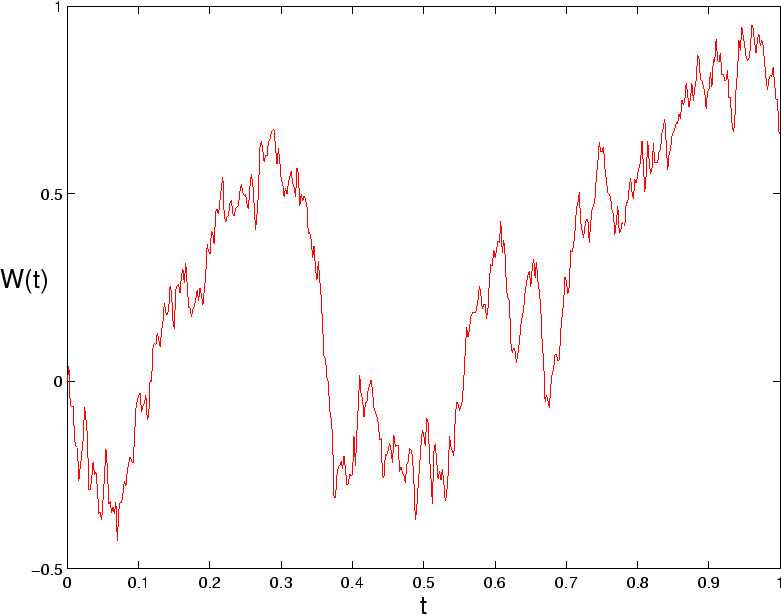
\includegraphics[scale=.3]{wiener-process}
			\captionof{figure}{A Wiener process \cite{wiener-process}}
			\label{fig:wiener-proc}
		\end{minipage} 
		
		The beginning of the use of fractals to describe landscapes did not coincide with the conception of the term "fractal" by Mandelbrot in the 1970s (see \autoref{sec:fractal}), but developed in the decades to come. This development in capturing surface topography was fueled by Mandelbrot's claim that all forms of nature can only be adequately described using fractals. While the potential of fractals to encapsulate and generate this geometry was noticed in the early 1990s, research at the time was still immature and unable to fully link the processes which create the forms captured by fractals. In terms of general landscapes, fractals were discovered to be able to imitate the self-similarity present in limited regions and limited ranges of scale in real landscapes. Some of the problems in furthering this research included the difficulty in researching and representing the dimensionality of natural terrain \cite{XU1993245}. Generating fractal structures ran into issues with processing time, causing a need for an alternative \cite{inbook}. However, this early PGC found its use in \emph{Star Trek II: The Wrath of Khan} \cite{startrek} to procedurally create imaginary planets. This technology was used later on in an accompaniment to a SIGGRAPH paper to demonstrate more of the ability of fractals. This set the stage for further use in movies such as \emph{The Last Starfighter} and \emph{Return of the Jedi} \cite{ibm-fractal}. 
		
		\section{Cellular Automata}
		
		During the development of fractals, cellular automata also were studied and gained traction. Cellular automata were originally proposed by John von Neumann, focusing on their structure in one and two dimensional grids. This idea was eventually extended into games by John Conway, with the motivation to design a simple set of rules to study the behavior of a population. By tuning different configurations, the "Game of Life" demonstrated a variety of growth patterns stemming from the initial population. Another example of the application of early cellular automata research to games was the \(\sigma(\sigma\textsuperscript{+})\) game, proposed by Sutner. This utilized the capabilities of cellular automata in a 2-d finite grid in order to have two players play against each other \cite{10.1145/349194.349202}.
		
		\section{Noise}
		
		In a similar period, Perlin noise was developed for use in the movie industry as well. It later became a foundation for many other procedural generation algorithms. It was developed in 1983 for use in the sci-fi movie Tron, to map textures onto computer generated surfaces for visual effects. Perlin noise has been used for many visual elements, ranging from the texture creation it was created for to particle effects such as fire, smoke and clouds, as well as landscapes and geological features. It has a variety of uses due to its ability to create a naturalistic appearance \cite{10.1145/325165.325247}.
		
		\section{Applications}
		One of the earliest usages of PGC in video games was in Rogue, in 1980 \cite{rogue}. This initial attempt at generating a dungeon in a random manner addressed some of the differences between procedural generation and purely random generation, by introducing some level of control to the designer. Rogue addressed this by using a three by three grid to generate the layout of the level, with hallways randomly connecting the rooms. These rooms would have a variable size to increase the variety of levels producible by the algorithm. This randomized methodology in particular, was created to address the memory constraints of computers at the time, as even with this more mathematical and less memory intensive approach, levels would need to be cleared from memory when moving on to the next one \cite{rogue}.
		
		% can add more here if have time...

		\section{Areas of Research}
	
		An ongoing area of research for PGC is the introduction of neural networks as the framework. One example of this is the procedural generation of terrain via Tensorflow. This implementation was trained on a large data-set of terrain height maps, around 10,000, with the addition of satellite data to use for coloring. The specific neural network involved in the implementation was a Generative Adversarial network\cite{goodfellow2014generative}, which works on creating fake images, and attempting to discern between real and fake. By iterating this, the network will get better at both tasks, with the generator learning how to create more and more realistic images. For the problem of coloring the terrain, a style network was used to take two images and blend them to create an output image that looks like the content image, but with the style of the reference image. Style networks are also used in other applications, such as the neural networks trained on recreating photographs in a particular artist's style, shown in \autoref{fig:neural-style}. 
		
		\begin{minipage}{\textwidth}
			\centering
			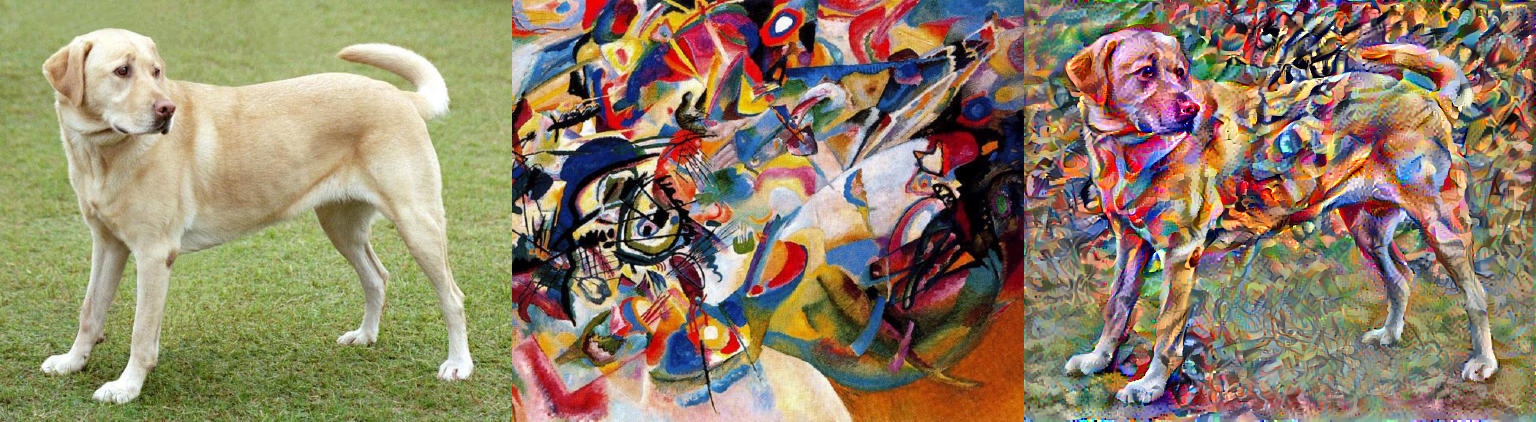
\includegraphics[scale=.3]{stylized-image}
			\captionof{figure}{An example of neural style transfer \cite{tf-style}}
			\label{fig:neural-style}
		\end{minipage}
	
		A kernel is part of image processing, and is applied to an image using convolutions. It is a \(n x n\) matrix, which is multiplied by over the pixels of an image, depending on the stride. \(n\) in this context provides the number of surrounding pixels, in a square formation for which to also draw values from for the new value of the pixel. The stride size refers to the distance the kernel moves for each convolution. If the stride size is too small, this can cause repeated multiplications across the image, a possible cause of artifacting. 
	
		\begin{minipage}{\textwidth}
			\centering
			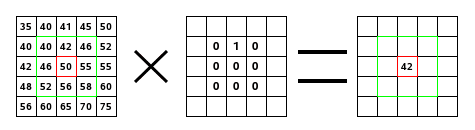
\includegraphics[scale=1]{convolution-calculate}
			\captionof{figure}{An of a kernel (pictured in the center as a 3x3 matrix) being multiplied at the target pixel in red. \cite{gimp}}
			\label{fig:gimp}
		\end{minipage}
		
		The initial processing pipeline for this image based deep learning algorithm utilized convolutional transpose to generate the output height and color-maps. However, this approach led to grid-like artifacting due to the misaligned output size compared to the kernel size. The solution used for combating this was bilinear sampling, by adding pixels from surrounding pixels to determine value rather than the kernels and strides. While the resultant height maps are impressive, additional research is likely required to determine differences between this approach and another approach such as Simplex noise. In \autoref{fig:dl-noise}, the results can be seen. 
		
		\begin{minipage}{\textwidth}
			\centering
			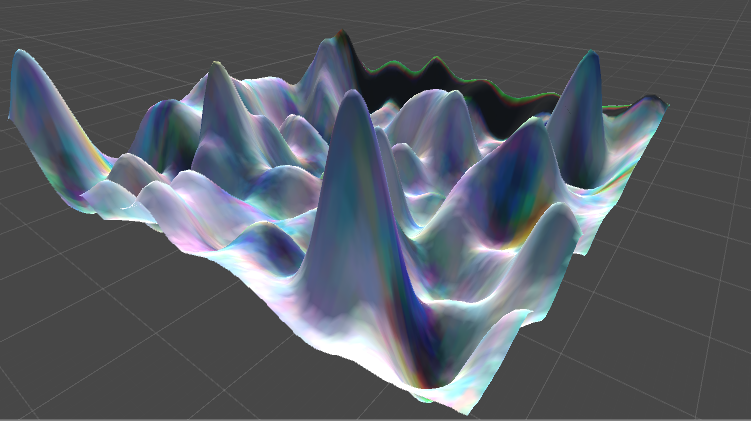
\includegraphics[scale=.3]{rolling}
			\captionof{figure}{Example of three-dimensional worlds created with deep learning \cite{nn-noise}}
			\label{fig:dl-noise}
		\end{minipage}
	
		The field of procedural content generation using machine learning is constantly evolving, as there are many different methodologies that have been applied to this task. The multitude of neural architectures allows for the tailoring of neural networks to different types of generated content, at the cost of necessitating large amounts of searching for the right architectures \cite{Liu_2020}.
		
		In addition to the advancements in noise generation, rendering associated with procedural generation have had advancements as well. For example voxel-based terrain has had advances in both the front and back-end of the algorithms. Voxel-based rendering methods often use a marching cubes algorithm to both smooth voxel surfaces and increase run-times. A modified version of this algorithm was created to facilitate faster implementation and design of a level-of-detail algorithm. Some of the difficulties of this revised implementation of the Marching Cubes algorithm involved finding a suitable compression for the voxel map, as for larger terrains, voxel mapping will quickly grow beyond the limits of addressable memory. In addition, limiting the density of vertices, triangles and individual meshes through a level-of-detail system ensures the higher rendering performance of this revised algorithm. 
		
		The modified Marching Cubes combined with a Transition Cubes algorithm provides a method for stitching together voxel-based meshes and eliminating seams. Rendering the areas of a terrain at different detail layers allows for efficient usage of processing power, but introduces the problem of seams between the cells. This problem can be shown in \autoref{fig:voxel-artifact}. 
		
		\begin{minipage}{\textwidth}
			\centering
			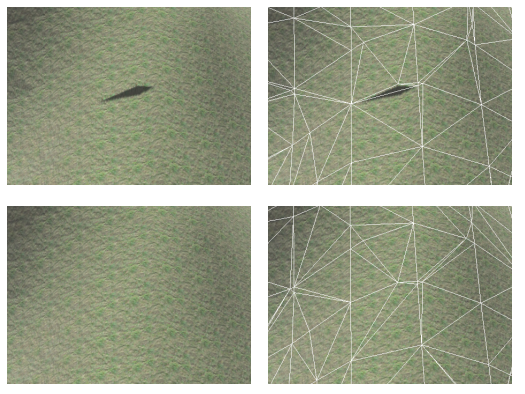
\includegraphics[scale=.75]{voxel-seam}
			\captionof{figure}{A shadow artifact fixed with transition cells \cite{10.5555/1925140}}
			\label{fig:voxel-artifact}
		\end{minipage}
		
		The Transition Cubes method developed in this paper utilizes transition cells inserted in between ordinary cells of a voxel map. This efficiently generates the triangles to connect terrain blocks rendered at different levels of detail, as modifications to one level of detail means that all levels must be adjusted to remain consistent, with the mapping of these different layers shown in \autoref{fig:voxel-layered-mapping}.
		
		\begin{minipage}{\textwidth}
			\centering
			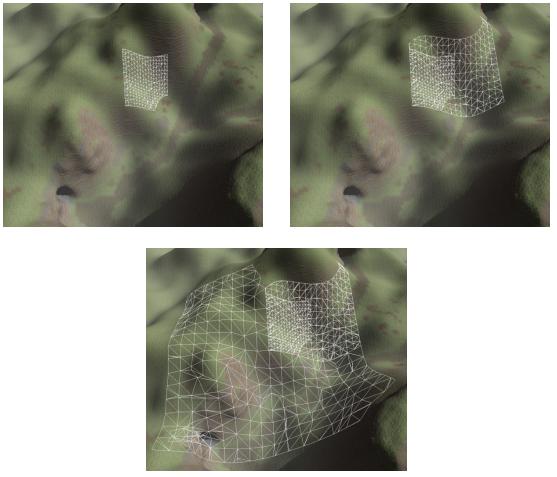
\includegraphics[scale=.75]{voxel-detail}
			\captionof{figure}{Layered resolution details of voxel meshes \cite{10.5555/1925140}}
			\label{fig:voxel-layered-mapping}
		\end{minipage}
		% URL holder http://transvoxel.org/Lengyel-VoxelTerrain.pdf
			
	\vspace{10pt}
	\let\clearpage\relax
	\chapter{Summary}
		
		While procedural generation has a background based in signals processing and fractal mathematics, its usage has extended far beyond these fields in the creation of PGC. Procedural algorithms are a useful way of automatically generating large amounts of data to interpret. The most well-known Noise-based procedural algorithm is Perlin noise, which generates n-dimensional noise from a n-dimensional lattice. Each lattice point has a pseudo-random gradient vector generated, and by interpolating the gradient vector with a unit distance vector, the value of the target point can be determined. To store the PGC, the procedural algorithm can be compartmentalized, or a height map can be created. To then render and interpret the procedurally created data, image based methods, polygonal methods, or voxels are all viable candidates. Perlin noise and other forms of procedural algorithms have had a long and varied development, with roots in fractal geometry, cellular automata, and signals. 
	
	\newpage
	\renewcommand{\bibname}{References}
	\bibliographystyle{plain}
	\bibliography{refs} % Entries are in the "refs.bib" file
		
\end{document}